% Phase 2 Learning Guide — personal study document, NOT a graded deliverable.
% Compile: xelatex Phase2_Learning_Guide.tex   (run twice for the table of contents)
\documentclass[11pt]{report}

\usepackage[margin=1in]{geometry}
\usepackage{amsmath}
\usepackage{amssymb}
\usepackage{fontspec}
\usepackage{graphicx}
\usepackage{booktabs}
\usepackage{longtable}
\usepackage{array}
\usepackage{xcolor}
\usepackage{caption}
\usepackage{enumitem}
\usepackage{tikz}
\usetikzlibrary{arrows.meta,positioning,shapes.geometric,fit,backgrounds,calc,matrix}
\usepackage{pgfplots}
\pgfplotsset{compat=1.18}
\usepackage[most]{tcolorbox}
\usepackage{listings}
\usepackage{titlesec}
\usepackage{fancyhdr}
\PassOptionsToPackage{hyphens}{url}
\usepackage[colorlinks=true,linkcolor=blue!50!black,urlcolor=blue!50!black,citecolor=blue!50!black]{hyperref}
\emergencystretch=3em
\sloppy

\newfontfamily\devanagarifont{Nirmala UI}
\newcommand{\dn}[1]{{\devanagarifont #1}}

\definecolor{hindiblue}{HTML}{1F6F8B}
\definecolor{nepalipurple}{HTML}{7A4FA3}
\definecolor{conceptgreen}{HTML}{2E8B57}
\definecolor{warnred}{HTML}{C0392B}
\definecolor{examplegold}{HTML}{B8860B}
\definecolor{codegray}{HTML}{F5F5F5}
\definecolor{titlenavy}{HTML}{102A43}

\titleformat{\chapter}[display]
  {\normalfont\huge\bfseries\color{titlenavy}}
  {\chaptertitlename\ \thechapter}{20pt}{\Huge}
\titleformat{\section}
  {\normalfont\Large\bfseries\color{titlenavy}}{\thesection}{1em}{}
\titleformat{\subsection}
  {\normalfont\large\bfseries\color{hindiblue}}{\thesubsection}{1em}{}

\pagestyle{fancy}
\fancyhf{}
\fancyhead[L]{\small\textit{Phase 2 Learning Guide}}
\fancyhead[R]{\small\leftmark}
\fancyfoot[C]{\thepage}
\renewcommand{\headrulewidth}{0.4pt}

\newtcolorbox{concept}[1]{colback=conceptgreen!6,colframe=conceptgreen,
  fonttitle=\bfseries,coltitle=white,colbacktitle=conceptgreen,
  title={\textbf{Concept: #1}},sharp corners=south,boxrule=1pt,left=2mm,right=2mm,breakable}

\newtcolorbox{implementation}[1]{colback=hindiblue!6,colframe=hindiblue,
  fonttitle=\bfseries,coltitle=white,colbacktitle=hindiblue,
  title={\textbf{In this project: #1}},sharp corners=south,boxrule=1pt,left=2mm,right=2mm,breakable}

\newtcolorbox{example}[1]{colback=examplegold!8,colframe=examplegold,
  fonttitle=\bfseries,coltitle=white,colbacktitle=examplegold,
  title={\textbf{Example: #1}},sharp corners=south,boxrule=1pt,left=2mm,right=2mm,breakable}

\newtcolorbox{notebox}[1][Note]{colback=gray!8,colframe=gray!60!black,
  fonttitle=\bfseries,left=2mm,right=2mm,title={\textbf{#1}},breakable}

\newtcolorbox{warnbox}[1][Watch out]{colback=warnred!8,colframe=warnred,
  fonttitle=\bfseries,coltitle=white,colbacktitle=warnred,
  left=2mm,right=2mm,title={\textbf{#1}},breakable}

\newtcolorbox{qabox}[1]{colback=nepalipurple!5,colframe=nepalipurple,
  fonttitle=\bfseries,coltitle=white,colbacktitle=nepalipurple,
  title={\textbf{Q: #1}},sharp corners=south,boxrule=1pt,left=2mm,right=2mm,
  breakable}

\lstset{
  backgroundcolor=\color{codegray},
  basicstyle=\ttfamily\small,
  breaklines=true,
  frame=single,
  rulecolor=\color{gray!50},
  showstringspaces=false,
  columns=fullflexible,
}

\newcommand{\p}[1]{\texttt{#1}}

\title{\Huge\textbf{Phase 2 — Complete Learning Guide}\\[0.3cm]
\Large Building, Training and Evaluating Two Transformers From Scratch\\[0.2cm]
\large Model H (Hindi) and Model L (Nepali), explained in plain words}
\author{Swaraj Kumar \\ \small 2025202016 \\[0.2cm]
\small \textit{Personal study document --- not a graded deliverable}}
\date{\today}

\begin{document}
\maketitle

\begin{tcolorbox}[colback=gray!8,colframe=gray!50!black,title={\textbf{What this document is, and how to use it}}]
This is a study guide I wrote for myself so that I can explain every part of my
Phase 2 work confidently in a viva. It is \textbf{not} a course deliverable and
does not affect grading --- the graded report is
\p{report/phase2/phase2\_report.md}.

Every number here comes from a file this project actually produced. Nothing is
invented. Where something was not done, or was done imperfectly, this guide says
so plainly --- because a viva examiner will find those places anyway, and it is
far better to walk in already knowing them.

\medskip
\textbf{If you are short on time:} read Chapter~\ref{ch:cheatsheet} (the cheat
sheet) and Chapter~\ref{ch:viva} (the question bank). Everything else exists to
make those two make sense.
\end{tcolorbox}

\tableofcontents

% =======================================================================
\chapter{What Phase 2 Actually Asked For}
% =======================================================================

\section{The assignment in one paragraph}

Phase 1 was about \emph{text}: collect a big pile of Hindi, collect a big pile of
Nepali, clean both, and train a tokenizer for each. Phase 2 is about
\emph{models}: take those two piles of text and train two separate neural
networks that can predict the next token. Write the network yourself, from basic
PyTorch pieces --- you are not allowed to import a ready-made Transformer.
Train both. Measure how good they are. Then look inside the attention heads and
describe what they learned.

That is the whole phase. Forty marks.

\section{The rules, and why each one exists}

\begin{longtable}{p{0.42\textwidth}p{0.52\textwidth}}
\toprule
\textbf{Rule} & \textbf{Why the course wants it} \\
\midrule
\endhead
Write the Transformer yourself from \p{nn.Linear}, \p{nn.Embedding},
\p{nn.LayerNorm}, \p{nn.Dropout}. No \p{nn.Transformer*}, no HuggingFace, no
pre-built attention block.
& So that you understand every tensor operation. You cannot explain a black box.
This is the entire point of the phase. \\
\addlinespace
Roughly 25M parameters per model.
& Small enough to train on a free GPU, large enough to actually learn something. \\
\addlinespace
Target about 500M training tokens per model.
& Gives each model enough data that the comparison between them is meaningful. \\
\addlinespace
Two \emph{completely independent} models: separate data, tokenizer, vocabulary,
weights.
& The whole scientific point is comparing a higher-resource language against a
lower-resource one. If they shared anything, the comparison would be
contaminated. \\
\addlinespace
Checkpoints must contain weights, optimizer state, scheduler state, step, and
config --- and training must resume from them.
& Free GPUs die without warning. A run you cannot resume is a run you can lose. \\
\addlinespace
Prove empirically that the model cannot see the future.
& Causal masking is easy to get subtly wrong, and a broken mask silently makes
every result meaningless. \\
\addlinespace
Report perplexity \emph{and} bits-per-byte.
& Perplexity depends on the tokenizer. Two models with different tokenizers
cannot be compared by perplexity alone. This turned out to be the most important
finding in my whole phase. \\
\addlinespace
Every plot needs a title, axis labels, and a legend.
& Plots without labels score zero for that component. \\
\bottomrule
\end{longtable}

\section{The eight things I had to hand in}

\begin{enumerate}[leftmargin=*]
\item The Transformer implementation (attention, positional embeddings, causal mask).
\item Model configuration files for both models.
\item Parameter counts, training scripts, and Drive links to the checkpoints.
\item Training logs and loss curves.
\item Perplexity / bits-per-byte tables, and BLEU, chrF, ROUGE-L.
\item Generated text samples plus diversity and repetition statistics.
\item Attention heatmaps plus entropy and distance summaries.
\item A written comparison of the two resource levels.
\end{enumerate}

Chapter~\ref{ch:compliance} checks all eight of these, strictly, against the
files that are actually in the repository.

% =======================================================================
\chapter{The Big Picture}
% =======================================================================

\section{What happens, end to end}

Before any of the details, here is the whole pipeline. Everything in this guide
is one of these boxes.

\begin{figure}[htbp]
\centering
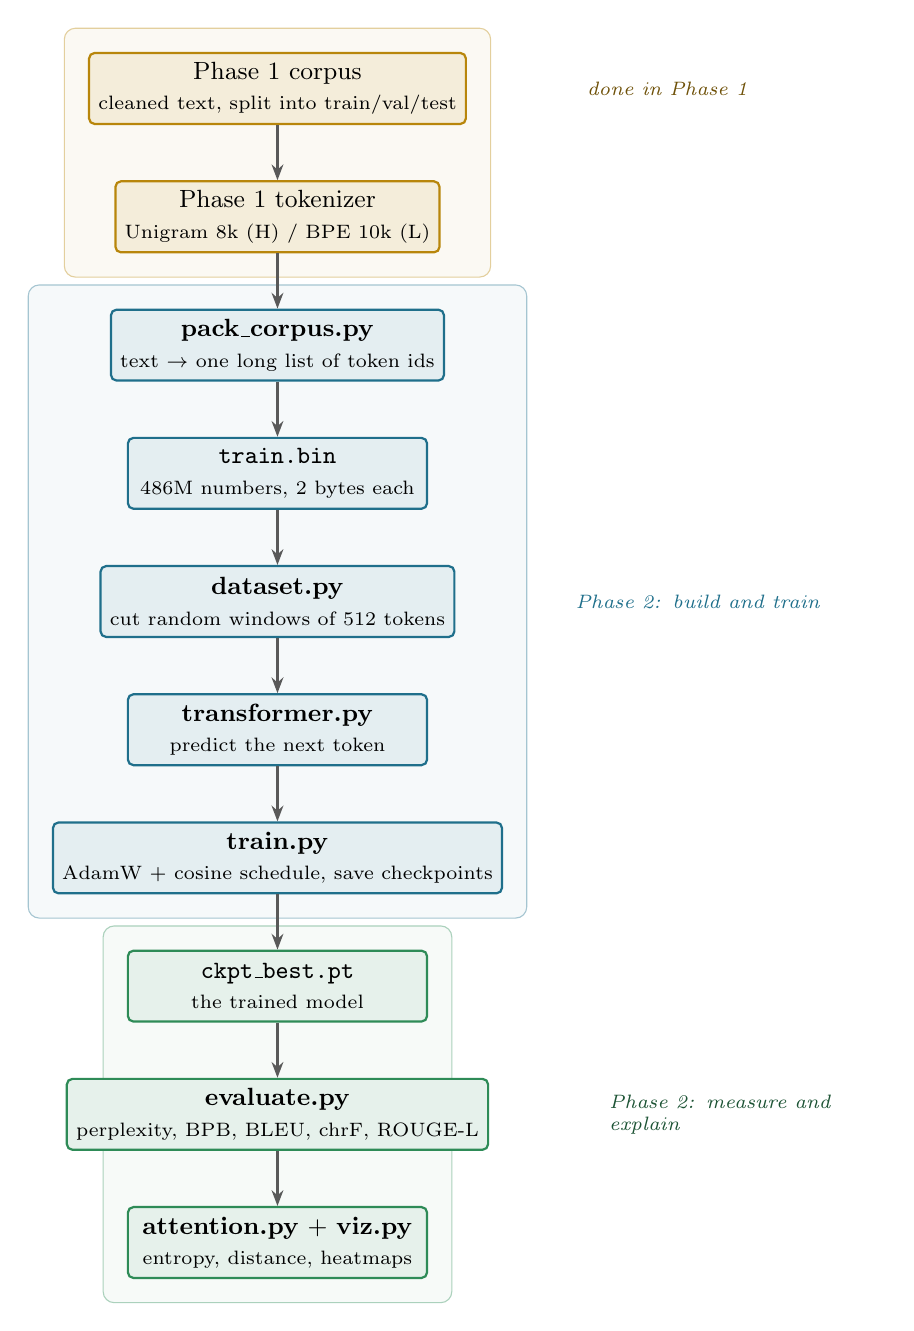
\begin{tikzpicture}[
  node distance=7mm,
  box/.style={draw,rounded corners=2pt,minimum width=38mm,minimum height=9mm,
              align=center,font=\small,thick},
  p1/.style={box,fill=examplegold!15,draw=examplegold},
  p2/.style={box,fill=hindiblue!12,draw=hindiblue},
  p3/.style={box,fill=conceptgreen!12,draw=conceptgreen},
  arr/.style={-{Stealth[length=2mm]},thick,gray!70!black}
]
\node[p1] (corpus) {Phase 1 corpus\\ \scriptsize cleaned text, split into train/val/test};
\node[p1,below=of corpus] (tok) {Phase 1 tokenizer\\ \scriptsize Unigram 8k (H) / BPE 10k (L)};
\node[p2,below=of tok] (pack) {\textbf{pack\_corpus.py}\\ \scriptsize text $\to$ one long list of token ids};
\node[p2,below=of pack] (bin) {\p{train.bin}\\ \scriptsize 486M numbers, 2 bytes each};
\node[p2,below=of bin] (batch) {\textbf{dataset.py}\\ \scriptsize cut random windows of 512 tokens};
\node[p2,below=of batch] (model) {\textbf{transformer.py}\\ \scriptsize predict the next token};
\node[p2,below=of model] (train) {\textbf{train.py}\\ \scriptsize AdamW + cosine schedule, save checkpoints};
\node[p3,below=of train] (ckpt) {\p{ckpt\_best.pt}\\ \scriptsize the trained model};
\node[p3,below=of ckpt] (eval) {\textbf{evaluate.py}\\ \scriptsize perplexity, BPB, BLEU, chrF, ROUGE-L};
\node[p3,below=of eval] (attn) {\textbf{attention.py} + \textbf{viz.py}\\ \scriptsize entropy, distance, heatmaps};

\foreach \a/\b in {corpus/tok,tok/pack,pack/bin,bin/batch,batch/model,model/train,train/ckpt,ckpt/eval,eval/attn}
  \draw[arr] (\a) -- (\b);

\node[right=14mm of corpus,font=\scriptsize\itshape,text width=34mm,align=left,examplegold!60!black]
  {done in Phase 1};
\node[right=14mm of batch,font=\scriptsize\itshape,text width=34mm,align=left,hindiblue]
  {Phase 2: build and train};
\node[right=14mm of eval,font=\scriptsize\itshape,text width=34mm,align=left,conceptgreen!60!black]
  {Phase 2: measure and explain};

\begin{scope}[on background layer]
  \node[fit=(corpus)(tok),draw=examplegold!40,fill=examplegold!5,rounded corners,inner sep=3mm]{};
  \node[fit=(pack)(train),draw=hindiblue!40,fill=hindiblue!4,rounded corners,inner sep=3mm]{};
  \node[fit=(ckpt)(attn),draw=conceptgreen!40,fill=conceptgreen!4,rounded corners,inner sep=3mm]{};
\end{scope}
\end{tikzpicture}
\caption{The Phase 2 pipeline. This exact chain ran twice --- once for Hindi,
once for Nepali --- with nothing shared between the two runs.}
\label{fig:pipeline}
\end{figure}

\begin{concept}{Why we convert text into a big list of numbers first}
Training reads data thousands of times. If every read had to open a text file
and run the tokenizer again, the GPU would sit idle waiting for the CPU.

So we tokenize \emph{once}, up front, and store the result as one enormous array
of numbers. Hindi's training split becomes 485,956,678 numbers in a single file.
Each number is stored in 2 bytes (\p{uint16}), which is enough because our
vocabularies are 8,000 and 10,000 --- both far below the 65,536 limit of a
2-byte number.

The file is about 972\,MB. During training we memory-map it, meaning the
operating system loads only the parts we touch, so we never need 972\,MB of RAM.
\end{concept}

\section{The two models, side by side}

\begin{center}
\begin{tabular}{lrr}
\toprule
& \textbf{Model H (Hindi)} & \textbf{Model L (Nepali)} \\
\midrule
Vocabulary & 8,000 (Unigram) & 10,000 (BPE) \\
Layers / heads / width & 6 / 8 / 512 & 6 / 8 / 512 \\
Feed-forward width & 2048 & 2048 \\
Context length & 512 & 512 \\
Total parameters & 23,273,472 & 24,297,472 \\
Non-embedding parameters & \textbf{18,915,328} & \textbf{18,915,328} \\
Training tokens & 475,791,360 & 473,169,920 \\
\bottomrule
\end{tabular}
\end{center}

\begin{implementation}{Why I made the two models identical on purpose}
Look at the non-embedding parameter counts: they are \emph{exactly} equal.
Look at the token counts: they differ by 0.55\%.

That was a deliberate design decision, and it is the single most important thing
to be able to justify in the viva. The whole point of the phase is to compare a
higher-resource language against a lower-resource one. If Model H also had more
layers, or trained on more tokens, then any difference in results could be
explained by "it was a bigger model" or "it trained longer" --- and the
comparison would prove nothing.

By making everything identical except the vocabulary (which \emph{has} to differ,
because the tokenizers differ), any difference that remains must come from the
data or the tokenizer. That is a clean experiment.
\end{implementation}

% =======================================================================
\chapter{Inside the Transformer, One Piece at a Time}
% =======================================================================

This is the chapter the viva will focus on hardest, because the whole point of
Phase 2 is that I wrote this myself. For every piece below I try to answer three
questions: \textbf{what does it compute}, \textbf{what shape is the tensor}, and
\textbf{what would break if it were removed}.

The code is \p{hindi/model/transformer.py} (and an identical, independent copy in
\p{nepali/model/transformer.py}).

\section{The shape notation, once}

\begin{center}
\begin{tabular}{cll}
\toprule
Symbol & Meaning & Our value \\
\midrule
$B$ & batch size --- how many sequences at once & 32 \\
$T$ & sequence length in tokens & 512 \\
$d$ & model dimension (width of each token's vector) & 512 \\
$h$ & number of attention heads & 8 \\
$d_k$ & width of one head, $= d/h$ & 64 \\
$V$ & vocabulary size & 8,000 (H) / 10,000 (L) \\
\bottomrule
\end{tabular}
\end{center}

\section{The whole model, drawn}

\begin{figure}[htbp]
\centering
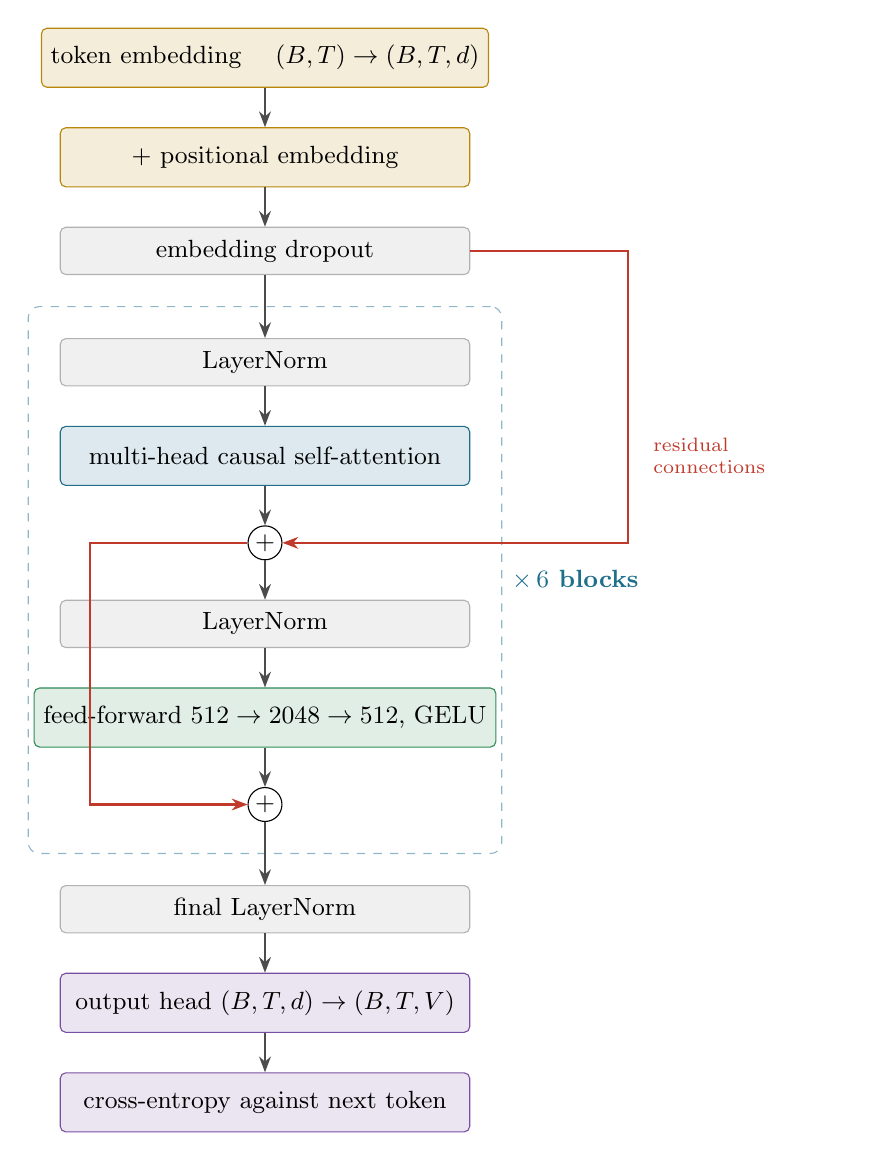
\begin{tikzpicture}[
  node distance=5mm,
  lay/.style={draw,rounded corners=2pt,minimum width=52mm,minimum height=7.5mm,
              align=center,font=\small},
  emb/.style={lay,fill=examplegold!15,draw=examplegold},
  att/.style={lay,fill=hindiblue!15,draw=hindiblue},
  ffn/.style={lay,fill=conceptgreen!15,draw=conceptgreen},
  nrm/.style={lay,fill=gray!12,draw=gray!60,minimum height=6mm},
  outbox/.style={lay,fill=nepalipurple!15,draw=nepalipurple},
  arr/.style={-{Stealth[length=2mm]},thick,gray!60!black},
  res/.style={-{Stealth[length=2mm]},thick,warnred}
]
\node[emb] (tok) {token embedding \quad $(B,T)\to(B,T,d)$};
\node[emb,below=of tok] (pos) {$+$ positional embedding};
\node[nrm,below=of pos] (drop) {embedding dropout};

\node[nrm,below=8mm of drop] (ln1) {LayerNorm};
\node[att,below=of ln1] (mha) {multi-head causal self-attention};
\node[circle,draw,below=of mha,inner sep=1pt,font=\small] (add1) {$+$};
\node[nrm,below=of add1] (ln2) {LayerNorm};
\node[ffn,below=of ln2] (ff) {feed-forward $512\to2048\to512$, GELU};
\node[circle,draw,below=of ff,inner sep=1pt,font=\small] (add2) {$+$};

\node[nrm,below=8mm of add2] (lnf) {final LayerNorm};
\node[outbox,below=of lnf] (head) {output head $(B,T,d)\to(B,T,V)$};
\node[outbox,below=of head] (loss) {cross-entropy against next token};

\foreach \a/\b in {tok/pos,pos/drop,drop/ln1,ln1/mha,mha/add1,add1/ln2,ln2/ff,ff/add2,add2/lnf,lnf/head,head/loss}
  \draw[arr] (\a) -- (\b);

\draw[res] (drop.east) -- ++(20mm,0) |- (add1.east);
\draw[res] (add1.west) -- ++(-20mm,0) |- (add2.west);

\node[right=22mm of mha,font=\scriptsize,text width=25mm,align=left,warnred]
  {residual\\ connections};

\begin{scope}[on background layer]
  \node[fit=(ln1)(add2),draw=hindiblue!50,dashed,rounded corners,inner sep=4mm,
        label={[font=\small\bfseries,hindiblue]right:$\times\,6$ blocks}]{};
\end{scope}
\end{tikzpicture}
\caption{The full forward pass. The dashed box is one Transformer block; we stack
six of them. Red lines are the residual connections that let gradients flow
straight down.}
\label{fig:arch}
\end{figure}

\section{Step 1 --- turning token ids into vectors}

\begin{concept}{Token embeddings}
A tokenizer gives us numbers like \p{[451, 12, 3987, ...]}. A number by itself
means nothing to a neural network --- token 451 is not "less than" token 452 in
any meaningful way.

So we keep a lookup table with one row per vocabulary entry: a matrix of shape
$(V, d) = (8000, 512)$. Token 451 becomes row 451, a list of 512 numbers. Those
512 numbers are \emph{learned} --- they start random and training adjusts them
until tokens that behave similarly end up with similar vectors.

Shape: $(B,T) \to (B,T,d)$, so $(32,512) \to (32,512,512)$.
\end{concept}

\section{Step 2 --- telling the model where each word is}

\begin{concept}{Why position has to be added separately}
This is the part people most often get asked about, and it has a neat answer.

Attention looks at every token and asks "how much should I care about every other
token?" But that computation treats the input as a \emph{bag} of tokens. It has
no idea which came first. If you shuffled the sentence, attention would produce
the same set of outputs, just shuffled --- the technical word is
\emph{permutation invariant}.

For language that is fatal. \dn{राम ने श्याम को देखा} (Ram saw Shyam) and
\dn{श्याम ने राम को देखा} (Shyam saw Ram) contain exactly the same tokens and
mean opposite things.

So we add a second lookup table, this one indexed by \emph{position} rather than
by token: position 0 gets a vector, position 1 gets a vector, and so on. We add
it to the token vector. Now the vector at position 5 carries both "which word"
and "where".
\end{concept}

\begin{implementation}{Learned absolute positions, and the price we pay}
I used \textbf{learned absolute} positional embeddings: a $(512, 512)$ table
that training adjusts, exactly like the token table.

The alternative was \emph{sinusoidal} encodings --- a fixed mathematical formula
of sines and cosines, not learned.

I chose learned because we train and evaluate at one fixed length (512), so the
main advantage of sinusoidal --- that it extends to lengths never seen --- buys
us nothing, while learned positions let the model spend capacity wherever the
data needs it.

\textbf{The price:} 512 is now a hard ceiling. There is literally no row 512 in a
512-row table, so the model cannot process a longer sequence. My \p{forward()}
raises a clear error rather than crashing with a confusing index error. If I ever
wanted longer context I would have to add rows and retrain, or interpolate the
table.

The code supports \p{sinusoidal} and \p{none} as config options too. \p{none} is
there for the optional bonus ablation (which I did not run --- see
Chapter~\ref{ch:compliance}).
\end{implementation}

\section{Step 3 --- multi-head causal self-attention}

This is the heart of the model. I will go through it slowly.

\subsection{The idea in one sentence}

Every token looks at all the tokens before it, decides how relevant each one is,
and pulls in a weighted mixture of their information.

\subsection{Queries, keys and values}

\begin{concept}{Q, K, V --- the library analogy}
Think of a library.

\begin{itemize}[leftmargin=*]
\item The \textbf{query} is what you are looking for: "I need something about
      irrigation."
\item Each book's \textbf{key} is its label on the spine: what it is about.
\item Each book's \textbf{value} is its actual contents.
\end{itemize}

You compare your query against every key to decide relevance, then take a
weighted blend of the contents of the relevant books.

In the model, every token produces all three, from the same input vector but
through three different learned matrices:
\[ Q = XW_Q, \qquad K = XW_K, \qquad V = XW_V \]
Each of $W_Q, W_K, W_V$ has shape $(d,d) = (512,512)$.
\end{concept}

\begin{implementation}{Three separate Linear layers, on purpose}
Many implementations fuse these into one big $(d, 3d)$ matrix and slice the
result --- it is slightly faster.

I deliberately kept \p{W\_q}, \p{W\_k}, \p{W\_v} as three separate
\p{nn.Linear} layers, because they then map one-to-one onto the $W_Q, W_K, W_V$
in the assignment's formula. If an examiner points at the equation and asks
"where is $W_K$ in your code", I can point at one line. That clarity was worth a
few percent of speed.
\end{implementation}

\subsection{Splitting into heads}

\begin{concept}{Why 8 heads instead of 1 big one}
One attention operation can really only learn one kind of relationship well. But
language has many relationships happening at once: which noun a verb agrees with,
which earlier word a pronoun refers to, which token simply came before.

So we split the 512-wide vector into 8 chunks of 64, and run attention
\emph{separately} in each chunk. Each head can specialise. At the end we glue the
8 outputs back into 512 and mix them with one more matrix, $W_O$.

Chapter~\ref{ch:attn} shows that this specialisation really did happen in my
models --- some heads became "look at the previous token" detectors, others look
far back.
\end{concept}

The reshape is the fiddly bit, and examiners like asking about it:

\begin{lstlisting}
q = self.W_q(x)                              # (B, T, d)
q = q.view(B, T, self.n_head, self.head_dim) # (B, T, h, d_k)  split
q = q.transpose(1, 2)                        # (B, h, T, d_k)  head axis first
...
y = y.transpose(1, 2)                        # (B, T, h, d_k)  put time back
y = y.contiguous().view(B, T, d)             # (B, T, d)       glue heads
\end{lstlisting}

\begin{warnbox}[Why contiguous() is needed]
\p{transpose} does not move any data. It only changes the \emph{strides} --- the
bookkeeping that says how far to step in memory for the next element. The numbers
stay where they were.

\p{view} requires the data to be laid out in one unbroken run in memory. After a
transpose it is not. So we call \p{contiguous()}, which physically copies the
data into the right order, and only then can we \p{view} it.

If you forget it, PyTorch raises an error telling you to call \p{contiguous()}.
It is a very common interview question.
\end{warnbox}

\subsection{Scaled dot-product attention}

For each head:
\[
\text{Attention}(Q,K,V) = \text{softmax}\!\left(\frac{QK^\top}{\sqrt{d_k}} + M\right)V
\]

Step by step, with shapes:

\begin{center}
\begin{tabular}{llp{0.42\textwidth}}
\toprule
Operation & Shape after & What it means \\
\midrule
$QK^\top$ & $(B,h,T,T)$ & every token's score against every other token \\
$\div \sqrt{d_k}$ & $(B,h,T,T)$ & keep the numbers a sensible size \\
$+ M$ & $(B,h,T,T)$ & block the future \\
softmax & $(B,h,T,T)$ & turn scores into probabilities that sum to 1 \\
$\times V$ & $(B,h,T,d_k)$ & weighted mixture of the value vectors \\
\bottomrule
\end{tabular}
\end{center}

\begin{concept}{Why divide by $\sqrt{d_k}$ --- guaranteed viva question}
At the start of training, the entries of $Q$ and $K$ are roughly random numbers
of size about 1. A dot product adds up $d_k = 64$ products of such numbers, so
the result has a typical size of about $\sqrt{64} = 8$ --- and in general it
grows like $\sqrt{d_k}$.

Now feed a set of numbers like $\{8, -8, 5\}$ into a softmax. The biggest one
wins overwhelmingly: the output is nearly $\{1, 0, 0\}$. That is called
\emph{saturation}, and a saturated softmax has almost zero gradient --- so
learning stops before it starts.

Dividing by $\sqrt{d_k}$ cancels exactly that growth and brings the scores back
to size $\approx 1$, where softmax is smooth and gradients flow.

\textbf{If you removed it:} the deeper or wider the model, the worse it would get.
Training would stall or diverge.
\end{concept}

\subsection{The causal mask}

\begin{concept}{Why the model must not see the future}
We train the model to predict the next token. If, while predicting position 5,
the model could look at position 6, it would just copy the answer. Loss would
drop to almost nothing and the model would learn nothing useful. At generation
time there \emph{is} no future to look at, so it would produce garbage.

So we block it. We build a matrix $M$ that is $0$ where looking is allowed and
$-\infty$ where it is not, and add it to the scores before the softmax.

Why $-\infty$ and not just a big negative number? Because
$e^{-\infty} = 0$ \emph{exactly}. The blocked positions get exactly zero
probability, not "very small" probability.
\end{concept}

\begin{figure}[htbp]
\centering
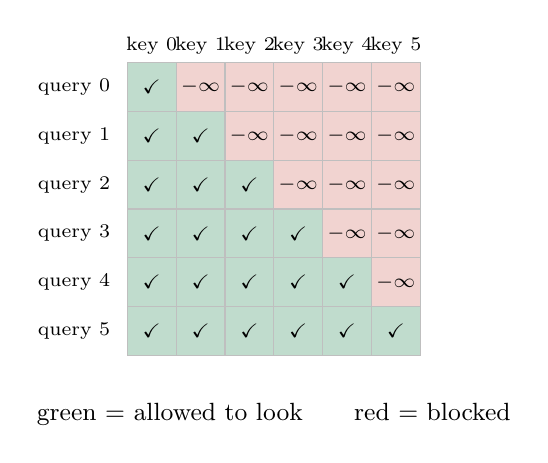
\begin{tikzpicture}[scale=0.62,every node/.style={font=\scriptsize}]
  \foreach \i in {0,...,5} {
    \foreach \j in {0,...,5} {
      \pgfmathparse{\j<=\i ? 1 : 0}
      \ifnum\pgfmathresult=1
        \fill[conceptgreen!30] (\j,-\i) rectangle ++(1,-1);
        \node at (\j+0.5,-\i-0.5) {\checkmark};
      \else
        \fill[warnred!22] (\j,-\i) rectangle ++(1,-1);
        \node at (\j+0.5,-\i-0.5) {$-\infty$};
      \fi
      \draw[gray!50] (\j,-\i) rectangle ++(1,-1);
    }
  }
  \foreach \j in {0,...,5} \node at (\j+0.5,0.35) {key \j};
  \foreach \i in {0,...,5} \node[anchor=east] at (-0.15,-\i-0.5) {query \i};
  \node[align=center,font=\small] at (3,-7.2)
    {green = allowed to look\qquad red = blocked};
\end{tikzpicture}
\caption{The causal mask for a 6-token sequence. Query 2 may look at keys 0, 1
and 2, but nothing after. This is an upper-triangular block of $-\infty$.}
\label{fig:mask}
\end{figure}

\begin{implementation}{How I proved the mask works}
The assignment specifically asks to \emph{show} that changing token $t{+}1$ does
not change the logits at position $t$. My test
(\p{hindi/tests/test\_model.py}) does exactly that:

\begin{enumerate}[leftmargin=*]
\item Run the model on a sequence, save all the logits.
\item For each position $t$: change every token after $t$ to something different.
\item Run again. Compare the logits at positions $\le t$.
\end{enumerate}

\textbf{Result: the maximum difference is $0.000\text{e}{+}00$.} Not "small" ---
exactly zero.

Why exactly zero and not just tiny? Because $\text{softmax}(-\infty)$ is exactly
$0$, and $0 \times v = 0$ exactly in floating-point arithmetic. The blocked
tokens contribute literally nothing.

The test also checks the \emph{opposite} direction: that the logits at positions
after $t$ \emph{did} change. Without that second check, a model that ignored its
input entirely would also pass.
\end{implementation}

\section{Step 4 --- the feed-forward network}

\begin{concept}{What the FFN is for}
Attention mixes information \emph{between positions}. The feed-forward network
mixes information \emph{within} one position --- it is applied to each token
separately and identically.

It is two linear layers with a non-linearity between them:
\[ 512 \xrightarrow{\ \text{expand}\ } 2048 \xrightarrow{\ \text{GELU}\ } 2048 \xrightarrow{\ \text{shrink}\ } 512 \]

Going wide in the middle gives the layer room to compute something complicated
before compressing back. This is where most of the model's parameters live.

I used GELU rather than ReLU because it is smooth around zero, which gives
better-behaved gradients for small models.
\end{concept}

\section{Step 5 --- residual connections and LayerNorm}

\begin{concept}{Residual connections: the road that skips}
Instead of \p{x = Attention(x)} we write \p{x = x + Attention(x)}.

Two reasons. First, each block only has to learn a \emph{change} to make, not
rebuild the whole representation --- much easier. Second, and more importantly,
gradients flowing backwards have a clean path straight down the $+$ signs. Without
residuals, the gradient would have to survive multiplication through every layer,
and would shrink to nothing.

\textbf{If you removed them:} a 6-layer model might still limp along; a 30-layer
one would not train at all.
\end{concept}

\begin{concept}{LayerNorm, and pre- versus post-norm}
LayerNorm takes one token's 512 numbers and rescales them to have mean 0 and
standard deviation 1, then applies a learned scale and shift. It keeps activations
in a sane range so nothing explodes.

Note it normalises \emph{each position separately} --- it never mixes information
across time, which is what keeps it compatible with causal masking.

Where you put it matters:
\begin{itemize}[leftmargin=*]
\item \textbf{Post-norm} (the original 2017 paper):
      \p{x = LayerNorm(x + Attention(x))}. The norm sits \emph{on} the residual
      highway.
\item \textbf{Pre-norm} (what I used):
      \p{x = x + Attention(LayerNorm(x))}. The norm sits on the \emph{branch};
      the highway stays clean.
\end{itemize}

I used pre-norm because that clean highway means gradients reach the early layers
undistorted, which makes training much more forgiving --- post-norm deep stacks
famously need careful learning-rate warmup or they diverge.
\end{concept}

\section{Step 6 --- the output head and weight tying}

After six blocks and a final LayerNorm, we map each token's 512 numbers to a
score for every word in the vocabulary: $(B,T,512) \to (B,T,8000)$.

\begin{concept}{Weight tying --- reusing one matrix twice}
The input embedding is a $(V, d)$ matrix: word $\to$ vector. The output head is a
$(d, V)$ matrix: vector $\to$ word scores. They are transposes of each other in
shape.

\emph{Weight tying} means using the same matrix for both.

\textbf{What it saves:} $V \times d$ parameters. For Hindi that is
$8000 \times 512 = 4{,}096{,}000$ --- about 18\% of the entire model. For Nepali,
$10000 \times 512 = 5{,}120{,}000$, about 21\%.

\textbf{Why it also makes sense:} it forces a word's "input meaning" and "output
meaning" to be the same vector, which is a reasonable thing to want.
\end{concept}

\section{Step 7 --- the loss}

\begin{concept}{Next-token prediction, concretely}
Take the sentence and shift it by one. The input is tokens $0 \ldots T-1$; the
target is tokens $1 \ldots T$. The model's prediction at position $t$ is scored
against the real token at position $t{+}1$.

In my \p{dataset.py} this is literally two slices of the same array:
\begin{lstlisting}
x = stream[o     : o + 512]      # inputs
y = stream[o + 1 : o + 1 + 512]  # targets: same window, shifted by one
\end{lstlisting}

Then cross-entropy compares the predicted distribution against the true token,
averaged over all $B \times T = 16{,}384$ positions in the batch. Every position
contributes a training signal --- that is what makes language modelling so
data-efficient.
\end{concept}

\begin{example}{The one sanity check that catches everything}
Before training, an untrained model should have no idea what comes next, so it
should spread probability evenly over all $V$ words. The loss for a uniform guess
over $V$ options is $\ln V$.

For Hindi, $\ln 8000 = 8.987$. My model's very first measured loss was
\textbf{8.98}.

That single number confirms the embeddings are initialised sensibly, the loss is
wired up correctly, and the vocabulary size matches. If it had been much higher,
something was broken; much lower, and the model was somehow seeing the answer.
\end{example}

% =======================================================================
\chapter{Counting the Parameters by Hand}
% =======================================================================

An examiner may well ask "where do your 23 million parameters come from?" Here is
the arithmetic, which you can reproduce on paper.

\section{One block at a time}

With $d = 512$ and $d_{ff} = 2048$:

\begin{center}
\begin{tabular}{llr}
\toprule
Part & Formula & Count \\
\midrule
$W_Q, W_K, W_V, W_O$ & $4 \times 512 \times 512$ & 1,048,576 \\
their biases & $4 \times 512$ & 2,048 \\
FFN expand & $512 \times 2048$ & 1,048,576 \\
FFN shrink & $2048 \times 512$ & 1,048,576 \\
FFN biases & $2048 + 512$ & 2,560 \\
two LayerNorms & $2 \times 2 \times 512$ & 2,048 \\
\midrule
\textbf{one block} & & \textbf{3,152,384} \\
\textbf{six blocks} & $6 \times 3{,}152{,}384$ & \textbf{18,914,304} \\
\bottomrule
\end{tabular}
\end{center}

\section{Adding the parts outside the blocks}

\begin{center}
\begin{tabular}{lrr}
\toprule
Part & Model H & Model L \\
\midrule
Six blocks & 18,914,304 & 18,914,304 \\
Final LayerNorm & 1,024 & 1,024 \\
Token embedding $(V \times 512)$ & 4,096,000 & 5,120,000 \\
Positional embedding $(512 \times 512)$ & 262,144 & 262,144 \\
Output head & \textit{0 --- tied} & \textit{0 --- tied} \\
\midrule
\textbf{Total} & \textbf{23,273,472} & \textbf{24,297,472} \\
\textbf{Non-embedding} & \textbf{18,915,328} & \textbf{18,915,328} \\
\bottomrule
\end{tabular}
\end{center}

\begin{notebox}[The number to remember]
The \emph{non-embedding} counts are identical: \textbf{18,915,328}. That is the
"thinking" part of the model. The only difference between the two models is the
size of the vocabulary lookup table, which is forced on us by Phase 1.

If asked "are your two models the same size?", the honest answer is: the compute
core is byte-for-byte identical; the totals differ by exactly
$2000 \times 512 = 1{,}024{,}000$ parameters, which is the extra 2,000 Nepali
vocabulary entries.
\end{notebox}

\section{Why 6 layers of width 512, and not something else}

\begin{implementation}{The depth/width trade-off I chose}
The target was "about 25M parameters". Many shapes hit that. I picked
$6 \times 512$ for these reasons:

\begin{itemize}[leftmargin=*]
\item \textbf{7 layers would overshoot.} $7 \times 3.15\text{M} + 4.1\text{M}
      = 26.4$M --- above target. Six lands at 23.3M, comfortably under.
\item \textbf{Depth buys composition.} Attention can only combine information
      one "hop" per layer. Multi-step relationships need several layers. A wide,
      shallow model cannot chain reasoning steps.
\item \textbf{Width is quadratically expensive.} Doubling $d$ multiplies the
      per-block cost by four, because every matrix is $d \times d$.
\item \textbf{Evidence from my own results.} The attention analysis
      (Chapter~\ref{ch:attn}) shows the interesting specialisation --- sharp local
      heads at layers 2--4, long-range heads at layer 5 --- only appears with
      depth. A 3-layer model would not have shown that structure.
\end{itemize}
\end{implementation}


% =======================================================================
\chapter{Training: How the Model Actually Learns}
% =======================================================================

Code: \p{hindi/train/train.py}.

\section{The loop, in words}

Repeat 15,000 times (we managed about 14,500 --- see below):

\begin{enumerate}[leftmargin=*]
\item Pick random starting points in the token stream, cut windows of 512 tokens.
\item Run them through the model, get a loss.
\item Work out how each parameter should change (backward pass).
\item Nudge every parameter a little (optimizer step).
\item Every 500 steps: check the loss on held-out validation data and save a
      checkpoint.
\end{enumerate}

\section{Choosing batches by random offset}

\begin{concept}{Why random windows instead of reading in order}
The token stream is one long sequence of 486 million numbers. To make a batch we
pick 32 random starting positions and take 512 tokens from each.

This means we never have to shuffle the giant file --- randomness comes from
\emph{where} we start reading. It also means a window can straddle the boundary
between two documents. That is fine and even useful: we put an end-of-document
(EOS) token between documents, and the model learns that EOS means "a new,
unrelated thing starts now".
\end{concept}

\section{AdamW, and why we do not decay every parameter}

\begin{concept}{What the optimizer does}
Plain gradient descent moves every parameter by the same learning rate. Adam is
smarter: it keeps a running average of each parameter's gradient (momentum) and of
its squared gradient (how noisy it is), and takes bigger steps for parameters with
small, consistent gradients.

The "W" in AdamW is \emph{decoupled weight decay}: gently pulling weights towards
zero to stop them growing too large, applied separately from the gradient step.
\end{concept}

\begin{implementation}{Decay only the matrices}
I apply weight decay only to parameters with 2 or more dimensions --- the
matrices. Biases, LayerNorm gains and embeddings get \emph{no} decay.

Why: weight decay is meant to regularise the linear mixing that matrices do.
Biases and LayerNorm gains set scales and offsets; shrinking them toward zero just
fights the job they are doing. This is standard practice and a good thing to be
able to justify.
\end{implementation}

\section{The learning-rate schedule}

\begin{figure}[htbp]
\centering
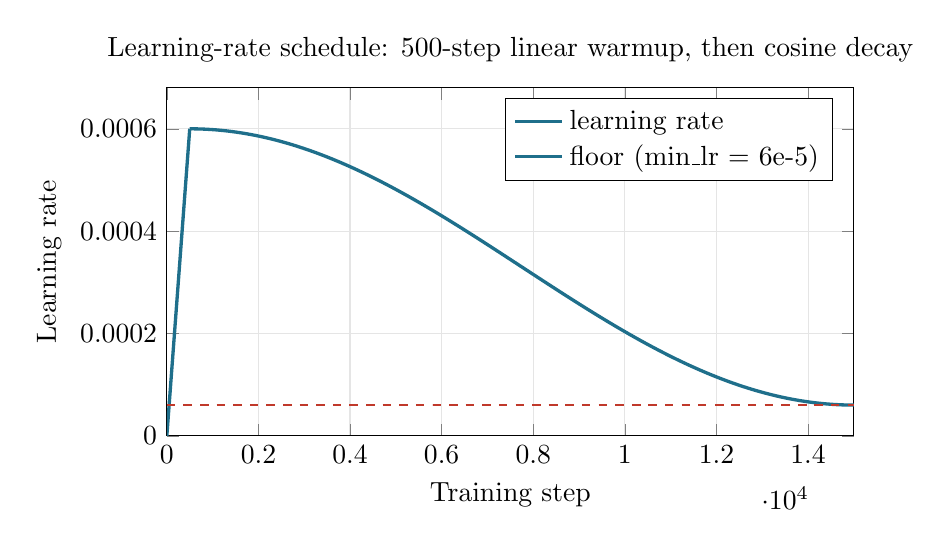
\begin{tikzpicture}
\begin{axis}[
  width=0.85\textwidth, height=6cm,
  title={Learning-rate schedule: 500-step linear warmup, then cosine decay},
  xlabel={Training step},
  ylabel={Learning rate},
  xmin=0, xmax=15000, ymin=0, ymax=6.8e-4,
  scaled y ticks=false,
  yticklabel style={/pgf/number format/fixed,/pgf/number format/precision=5},
  grid=both, grid style={gray!20},
  legend pos=north east, legend cell align=left,
  samples=200
]
\addplot[hindiblue,very thick,domain=0:500] {6e-4*x/500};
\addplot[hindiblue,very thick,domain=500:15000]
  {6e-5 + 0.5*(1+cos(deg(pi*(x-500)/14500)))*(6e-4-6e-5)};
\addlegendentry{learning rate}
\addplot[warnred,dashed,thick,domain=0:15000] {6e-5};
\addlegendentry{floor (min\_lr = 6e-5)}
\end{axis}
\end{tikzpicture}
\caption{The learning rate rises linearly for 500 steps, then follows a cosine
curve down to a floor of 6e-5. My final logged learning rate was 6.15e-05,
sitting just above the floor exactly as designed.}
\label{fig:lr}
\end{figure}

\begin{concept}{Why warmup, and why cosine}
\textbf{Warmup.} Adam needs a few hundred steps to build reliable estimates of
gradient noise. Taking full-size steps before then is a classic cause of early
divergence. So we ramp the learning rate up from nearly zero over 500 steps.

\textbf{Cosine decay.} Early in training, big steps make fast progress. Later,
big steps just bounce around the minimum. Cosine decay spends most of the budget
at a high rate then anneals smoothly, which reliably beats a fixed rate or a
sudden drop.
\end{concept}

\section{Gradient accumulation --- a big batch on a small GPU}

\begin{concept}{Faking a larger batch}
I wanted an effective batch of 32,768 tokens. That is
$32 \text{ sequences} \times 512 \text{ tokens} \times 2$.

Why the $\times 2$? Because instead of doing one giant forward/backward pass, I do
\emph{two} passes of 32 sequences each, adding up the gradients, and only then take
one optimizer step. The mathematics is the same as one batch of 64, but peak
memory is only that of 32.

This is the knob that decouples "the batch size the maths sees" from "what fits in
the GPU". On a smaller GPU I would lower \p{batch\_size} and raise
\p{grad\_accum\_steps} to keep the product the same.

One detail: I divide each micro-batch loss by the number of accumulation steps, so
the accumulated gradient is an \emph{average} rather than a sum.
\end{concept}

\section{Mixed precision}

\begin{concept}{float16, and why it needs a "gradient scaler"}
Doing arithmetic in 16-bit instead of 32-bit is roughly twice as fast and uses
half the memory. But 16-bit numbers have a small range, and gradients are tiny ---
many would round to zero and be lost.

The fix is a \emph{gradient scaler}: multiply the loss by a big number (say 65536)
before the backward pass, so gradients land in a representable range; then divide
them back before the optimizer step. If anything overflows, the scaler notices,
skips that step, and lowers the multiplier.

\textbf{bfloat16} would avoid all this, because it has the same exponent range as
float32. But Kaggle's T4 GPU is too old to support bfloat16, so my code detects
that and falls back to float16 with the scaler automatically.
\end{concept}

\section{Checkpointing --- the requirement that saved me}

\begin{implementation}{What is in a checkpoint, and why each piece matters}
\begin{center}
\begin{tabular}{ll}
\toprule
Saved & Why you need it to resume properly \\
\midrule
model weights & obvious --- the learned parameters \\
optimizer state & Adam's momentum estimates; losing them causes a loss spike \\
scheduler state & so the learning rate continues, not restarts \\
step number & so you know where you are \\
tokens consumed & for accurate logging and plots \\
best validation loss & so "best" stays meaningful across restarts \\
full config & so the model can be rebuilt with the right shape \\
RNG states & so the data order continues identically \\
\bottomrule
\end{tabular}
\end{center}

I verified resume across three consecutive sessions (12 $\to$ 18 $\to$ 24 steps)
\emph{before} starting the real runs. That test paid for itself immediately.
\end{implementation}

\begin{warnbox}[A real bug the resume test caught]
When I resumed with a larger \p{max\_steps}, the learning-rate schedule restored
its \emph{horizon} from the checkpoint too. So the schedule still thought it was
finishing at the old step count, computed "progress $>$ 100\%", and pinned the
learning rate at the floor for the entire extension.

Training would have looked like it had silently stalled --- loss barely moving,
no error message.

The fix: restore only the schedule's \emph{progress} (which step we are on) and
take its \emph{shape} (peak, floor, warmup, horizon) from the live config. The
code prints a line whenever the two disagree, so the change is never silent.

This is an excellent thing to mention in a viva --- it shows the resume path was
genuinely tested, not just written.
\end{warnbox}

\section{What actually happened during training}

\begin{figure}[htbp]
\centering
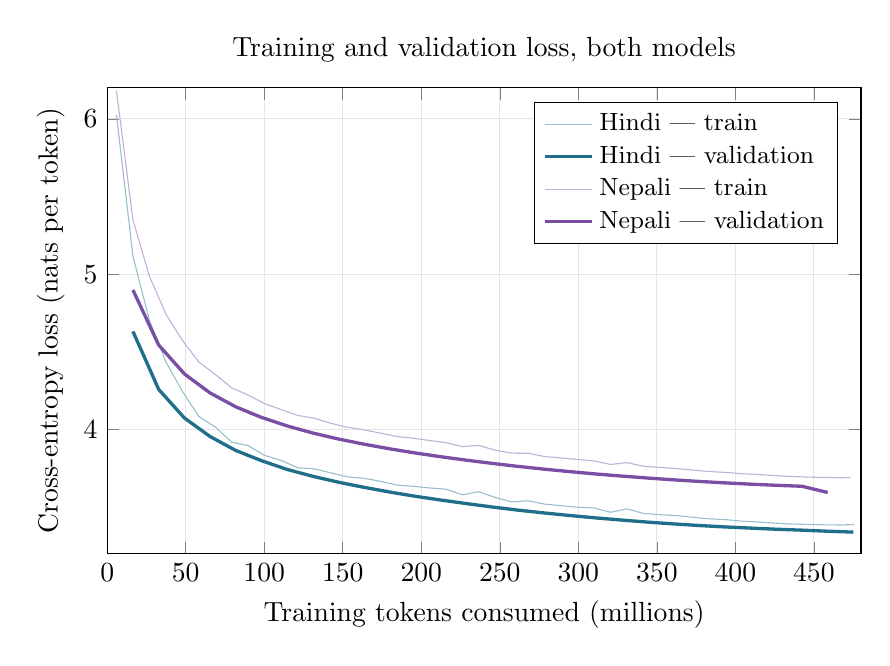
\begin{tikzpicture}
\begin{axis}[
  width=0.92\textwidth, height=7.5cm,
  title={Training and validation loss, both models},
  xlabel={Training tokens consumed (millions)},
  ylabel={Cross-entropy loss (nats per token)},
  xmin=0, xmax=480, ymin=3.2, ymax=6.2,
  grid=both, grid style={gray!20},
  legend pos=north east, legend cell align=left, legend style={font=\small}
]
\addplot[hindiblue!45,thin] coordinates{
(5.9,6.0263)(16.4,5.1161)(26.9,4.7036)(37.4,4.4354)(47.8,4.2476)(58.3,4.0855)
(68.8,4.0173)(79.3,3.9187)(89.8,3.8966)(100.3,3.8338)(110.8,3.8019)(121.2,3.7546)
(131.7,3.7476)(142.2,3.7223)(152.7,3.6960)(163.2,3.6873)(173.7,3.6678)(184.2,3.6434)
(194.6,3.6354)(205.1,3.6244)(215.6,3.6169)(226.1,3.5801)(236.6,3.6004)(247.1,3.5631)
(257.6,3.5347)(268.0,3.5419)(278.5,3.5206)(289.0,3.5103)(299.5,3.5003)(310.0,3.4957)
(320.5,3.4679)(331.0,3.4896)(341.4,3.4609)(351.9,3.4525)(362.4,3.4468)(372.9,3.4356)
(383.3,3.4257)(393.8,3.4206)(404.3,3.4104)(414.8,3.4051)(425.2,3.3980)(435.7,3.3921)
(446.2,3.3899)(456.7,3.3871)(467.1,3.3860)(475.8,3.3893)};
\addlegendentry{Hindi --- train}
\addplot[hindiblue,very thick] coordinates{
(16.4,4.6321)(32.8,4.2588)(49.2,4.0745)(65.5,3.9556)(81.9,3.8656)(98.3,3.7999)
(114.7,3.7433)(131.1,3.6989)(147.5,3.6610)(163.8,3.6280)(180.2,3.5977)(196.6,3.5701)
(213.0,3.5459)(229.4,3.5228)(245.8,3.5011)(262.1,3.4810)(278.5,3.4633)(294.9,3.4468)
(311.3,3.4315)(327.7,3.4176)(344.1,3.4046)(360.4,3.3931)(376.8,3.3828)(393.2,3.3736)
(409.6,3.3660)(426.0,3.3588)(442.4,3.3527)(458.8,3.3459)(475.1,3.3402)};
\addlegendentry{Hindi --- validation}
\addplot[nepalipurple!45,thin] coordinates{
(5.9,6.1802)(16.4,5.3496)(26.9,4.9877)(37.4,4.7434)(47.8,4.5760)(58.3,4.4360)
(68.8,4.3552)(79.3,4.2687)(89.8,4.2222)(100.3,4.1673)(110.8,4.1289)(121.2,4.0916)
(131.7,4.0742)(142.2,4.0409)(152.7,4.0159)(163.2,3.9990)(173.7,3.9783)(184.2,3.9560)
(194.6,3.9448)(205.1,3.9299)(215.6,3.9160)(226.1,3.8907)(236.6,3.8983)(247.1,3.8677)
(257.6,3.8484)(268.0,3.8478)(278.5,3.8265)(289.0,3.8176)(299.5,3.8079)(310.0,3.7981)
(320.5,3.7758)(331.0,3.7876)(341.4,3.7644)(351.9,3.7570)(362.4,3.7492)(372.9,3.7398)
(383.3,3.7301)(393.8,3.7245)(404.3,3.7159)(414.8,3.7104)(425.2,3.7038)(435.7,3.6982)
(446.2,3.6944)(456.7,3.6920)(467.1,3.6903)(473.2,3.6912)};
\addlegendentry{Nepali --- train}
\addplot[nepalipurple,very thick] coordinates{
(16.4,4.8990)(32.8,4.5443)(49.2,4.3585)(65.5,4.2361)(81.9,4.1466)(98.3,4.0784)
(114.7,4.0233)(131.1,3.9776)(147.5,3.9389)(163.8,3.9058)(180.2,3.8759)(196.6,3.8489)
(213.0,3.8247)(229.4,3.8024)(245.8,3.7818)(262.1,3.7627)(278.5,3.7452)(294.9,3.7291)
(311.3,3.7143)(327.7,3.7008)(344.1,3.6883)(360.4,3.6769)(376.8,3.6665)(393.2,3.6572)
(409.6,3.6489)(426.0,3.6416)(442.4,3.6353)(458.8,3.5953)};
\addlegendentry{Nepali --- validation}
\end{axis}
\end{tikzpicture}
\caption{Both models trained on almost identical token budgets. Validation loss
(thick) falls monotonically to the end for both --- no overfitting, and both would
likely keep improving with more compute. Curves reconstructed from the committed
training logs.}
\label{fig:loss}
\end{figure}

\begin{notebox}[Reading this plot in a viva]
Three things to point out:

\textbf{1. Validation is below training.} That looks odd but is expected: dropout
is \emph{on} during training and \emph{off} during evaluation, so the training
number is measured on a deliberately handicapped model.

\textbf{2. No gap opening up.} If the model were overfitting, validation loss
would flatten or turn upward while training loss kept falling. Neither does. With
23M parameters and 476M tokens we are nowhere near memorising the data.

\textbf{3. Both curves are still descending at the end.} More compute would have
given better models. We stopped because of a time budget, not because we
converged.
\end{notebox}

\begin{warnbox}[Honest limitation: we did not finish all 15,000 steps]
Planned: 15,000 steps. Actual: 14,520 (Hindi) and 14,440 (Nepali).

Why: the measured throughput was 12.0k tokens/second, slower than I had projected,
so the notebook's 11-hour safety budget fired first. It exited cleanly and wrote a
resumable checkpoint, then went on to run the evaluation.

Why it does not damage the comparison: the two budgets differ by only 0.55\%, so
the models are still on equal footing. I report what actually ran, not what was
planned.
\end{warnbox}

% =======================================================================
\chapter{Evaluation: How Good Are They?}
% =======================================================================

Code: \p{hindi/eval/evaluate.py}.

\section{Cross-entropy and perplexity}

\begin{concept}{Perplexity in plain words}
Cross-entropy is the average "surprise" of the model, in nats. Perplexity is just
$e^{\text{cross-entropy}}$, and it has a nice interpretation:

\textbf{perplexity is roughly how many options the model is effectively choosing
between at each step.}

A perplexity of 27 means the model is about as uncertain as if it were picking
uniformly among 27 words. Compare that to picking among all 8,000 --- it has
learned a great deal.
\end{concept}

\begin{center}
\begin{tabular}{lrr}
\toprule
& \textbf{Model H (Hindi)} & \textbf{Model L (Nepali)} \\
\midrule
Validation cross-entropy & 3.2985 & 3.8317 \\
Validation perplexity & \textbf{27.07} & 46.14 \\
Test cross-entropy & 3.3109 & 3.8433 \\
Test perplexity & \textbf{27.41} & 46.68 \\
\bottomrule
\end{tabular}
\end{center}

\section{Bits-per-byte, and the most important finding in my project}

\begin{warnbox}[The trap perplexity sets]
Looking at the table above you would say: Model H is far better, by 41\%.

That conclusion is \textbf{wrong}, or at least badly incomplete --- and knowing
why is the single most valuable thing I can bring into the viva.
\end{warnbox}

\begin{concept}{Why perplexity cannot compare two different tokenizers}
Perplexity is measured \emph{per token}. But a "token" is not the same amount of
text in the two models.

\begin{center}
\begin{tabular}{lrr}
\toprule
& Model H & Model L \\
\midrule
Tokenizer & Unigram 8,000 & BPE 10,000 \\
\textbf{Bytes of text per token} & \textbf{8.88} & \textbf{11.44} \\
\bottomrule
\end{tabular}
\end{center}

Nepali's tokens carry 29\% more text each. Bigger chunks are harder to guess ---
predicting a whole word is harder than predicting half a word. So Model L is
being asked a harder question at every step, and its perplexity looks worse for
that reason alone.

It is like comparing two students where one is asked to guess the next
\emph{letter} and the other the next \emph{word}, then concluding the second is
worse because they get more wrong.
\end{concept}

\begin{concept}{Bits-per-byte fixes it}
Instead of dividing the total surprise by the number of \emph{tokens}, divide it
by the number of \emph{bytes} of actual text. Now the unit is the same for both
models, and the tokenizer cancels out.

\[
\text{BPB} = \frac{\text{total surprise in bits}}{\text{total bytes of text}}
\]

Worked out for my two models:
\begin{align*}
\text{Model H:} \quad & 3.3109 \text{ nats} \div \ln 2 = 4.777 \text{ bits/token},
  \quad 4.777 \div 8.88 = \mathbf{0.5382} \text{ BPB} \\
\text{Model L:} \quad & 3.8433 \text{ nats} \div \ln 2 = 5.545 \text{ bits/token},
  \quad 5.545 \div 11.44 = \mathbf{0.4846} \text{ BPB}
\end{align*}
\end{concept}

\begin{figure}[htbp]
\centering
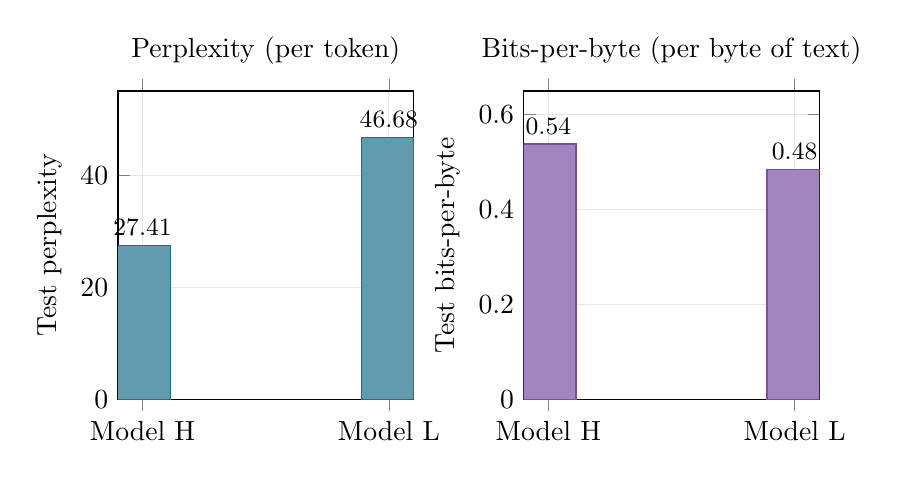
\begin{tikzpicture}
\begin{axis}[
  name=left,
  width=0.44\textwidth, height=5.5cm,
  title={Perplexity (per token)},
  ybar, bar width=20pt,
  symbolic x coords={Model H, Model L},
  xtick=data, ymin=0, ymax=55,
  ylabel={Test perplexity}, nodes near coords,
  every node near coord/.append style={font=\small},
  grid=major, grid style={gray!20},
]
\addplot[fill=hindiblue!70,draw=hindiblue] coordinates {(Model H,27.41) (Model L,46.68)};
\end{axis}
\begin{axis}[
  at={(left.east)}, anchor=west, xshift=14mm,
  width=0.44\textwidth, height=5.5cm,
  title={Bits-per-byte (per byte of text)},
  ybar, bar width=20pt,
  symbolic x coords={Model H, Model L},
  xtick=data, ymin=0, ymax=0.65,
  ylabel={Test bits-per-byte}, nodes near coords,
  every node near coord/.append style={font=\small},
  grid=major, grid style={gray!20},
]
\addplot[fill=nepalipurple!70,draw=nepalipurple] coordinates {(Model H,0.5382) (Model L,0.4846)};
\end{axis}
\end{tikzpicture}
\caption{The same two models, two metrics, opposite conclusions. Perplexity says
Model H wins comfortably. Bits-per-byte --- which removes the tokenizer from the
comparison --- puts Model L marginally ahead. Lower is better in both plots.}
\label{fig:pplbpb}
\end{figure}

\begin{notebox}[What this does and does not mean]
\textbf{It does not mean Model L is the better language model.} The difference in
BPB is small.

\textbf{It does mean the 41\% perplexity gap is mostly an artifact of the
tokenizer, not a real quality gap.} Had I reported perplexity alone, I would have
concluded that the lower-resource language produced a substantially worse model.
The tokenizer-neutral metric says they are close.

That is exactly why the assignment asks for BPB "to make the two languages more
comparable when tokenizers differ" --- and my results demonstrate the point
rather than just restating it.
\end{notebox}

\begin{warnbox}[One caveat to state before anyone else does]
BPB looks unusually low for both models. That is because Devanagari costs
\textbf{three UTF-8 bytes per character}, which inflates the denominator.

So these BPB numbers are comparable \emph{Hindi against Nepali} --- both
Devanagari --- but must \emph{not} be compared against an English model, where
most characters cost one byte. Saying "my model gets 0.48 BPB, better than
GPT-2's" would be nonsense.
\end{warnbox}

\section{Generation metrics}

We take 64 real prefixes from the held-out set, ask the model to continue them,
and compare against what actually came next.

\begin{center}
\begin{tabular}{llrrrrr}
\toprule
Model & Decoding & BLEU-4 & chrF++ & ROUGE-L & Repetition & Distinct-1 \\
\midrule
H & greedy & 1.96 & 12.49 & 0.093 & 0.598 & 0.172 \\
H & $T=0.5$ & 1.80 & 14.33 & 0.096 & 0.212 & 0.275 \\
H & $T=1.0$ & 1.01 & \textbf{16.29} & 0.100 & 0.002 & 0.520 \\
H & $T=1.5$ & 0.16 & 14.67 & 0.053 & 0.000 & 0.702 \\
\midrule
L & greedy & 2.37 & 14.48 & 0.081 & 0.577 & 0.179 \\
L & $T=0.5$ & 1.88 & 16.54 & 0.092 & 0.190 & 0.345 \\
L & $T=1.0$ & 1.69 & \textbf{18.05} & 0.079 & 0.001 & 0.634 \\
L & $T=1.5$ & 0.78 & 16.13 & 0.035 & 0.000 & 0.793 \\
\bottomrule
\end{tabular}
\end{center}

\begin{concept}{What temperature does}
Temperature reshapes the probability distribution before we sample from it.

\begin{itemize}[leftmargin=*]
\item \textbf{Greedy} --- always take the single most likely token. Sounds
      sensible; in practice it gets stuck in loops.
\item \textbf{$T < 1$} --- sharpen. Safer, more repetitive.
\item \textbf{$T = 1$} --- sample from the model's actual distribution.
\item \textbf{$T > 1$} --- flatten. More variety, less coherence.
\end{itemize}
\end{concept}

\begin{concept}{Why each metric is or is not useful here --- the assignment asks this}
\textbf{BLEU-4} counts exact 4-word matches against \emph{one} reference. But
there are a thousand valid ways to continue a sentence, and the model's is
unlikely to match the one true continuation word-for-word. So BLEU is near the
floor (0.16--2.37) and should not be read as a quality score. It is only useful
\emph{relatively}, comparing settings of the same model. It is the weakest of the
three here.

\textbf{chrF / chrF++} compare \emph{character} n-grams. That matters enormously
for Hindi and Nepali, which are heavily inflected --- \dn{घर}, \dn{घरमा},
\dn{घरहरू} are different words to BLEU but share most characters. chrF also needs
no word tokenizer. \textbf{This is the metric I trust most}, and notably it peaks
at $T=1.0$, which is also where the text reads best.

\textbf{ROUGE-L} finds the longest common subsequence, so it is more forgiving
about word order than BLEU. I implemented it myself rather than using the standard
\p{rouge\_score} library, because that library's default tokenizer lowercases and
strips non-ASCII characters --- which would delete Devanagari entirely and
silently report zero. That is a subtle trap worth mentioning.
\end{concept}

\section{Repetition and diversity --- where the models visibly fail}

\begin{example}{Greedy decoding falls apart}
\textbf{Model H, greedy} --- gets stuck:
\begin{quote}\dn{...इस सिद्धान्त के अनुसार, "अर्थात्, अष्टांग, अष्टांग, अष्टांग...}\end{quote}

\textbf{Model H, $T=0.5$} --- still stuck, different word:
\begin{quote}\dn{...उस पर चिन्तन कर सकने वाला साधक साधक साधक साधक...}\end{quote}

\textbf{Model L, greedy} --- repeats a whole phrase:
\begin{quote}\dn{...कृषि अनुदानको व्यवस्था गर्न जरुरी छ । कृषि अनुदानको व्यवस्था गर्न जरुरी छ ।...}\end{quote}

\textbf{Model L, $T=0.5$} --- coherent and on-topic:
\begin{quote}\dn{..., ब्याज, ब्याज, अनुदान, कृषि ऋण आदिको व्यवस्था गर्नु आवश्यक छ । तर, यो नीतिले कृषिको उत्पादकत्व...}\end{quote}
\end{example}

\begin{concept}{Why greedy decoding degenerates}
Once the model outputs a word, that word is now in its own context, which makes
the same word slightly more likely next time. Greedy decoding always takes the
maximum, so the loop tightens and never escapes. Sampling breaks the cycle,
because there is always a chance of picking something else.

The numbers say it clearly: greedy repeats \textbf{59.8\%} of its 4-grams
(Model H). At $T=1.0$ that drops to \textbf{0.2\%}.
\end{concept}

\begin{notebox}[The clean result to quote]
Going from greedy to $T=1.0$ removes essentially all repetition \emph{and}
improves chrF++ at the same time (12.49 $\to$ 16.29 for Model H). So for these
models, up to $T=1.0$, the diversity gain costs nothing in quality. Beyond that
($T=1.5$) chrF++ falls again and the text stops being grammatical.

Diversity and quality are not always a trade-off --- here there was free lunch up
to a point, and the metrics locate that point.
\end{notebox}

\textbf{Qualitative honesty:} both models produce well-formed Devanagari with
correct conjuncts and plausible grammar at $T \le 1.0$. Neither keeps a coherent
topic beyond roughly one sentence. That is entirely expected for 23M parameters
trained on 476M tokens --- these are small models by modern standards.


% =======================================================================
\chapter{Looking Inside the Attention Heads}
\label{ch:attn}
% =======================================================================

Because I implemented attention myself, I can pull out the actual probability
matrices and ask what the heads learned. Code: \p{hindi/eval/attention.py}.

\section{The two measurements}

\begin{concept}{Attention entropy --- is this head focused or vague?}
Each query position produces a probability distribution over the tokens it can
see. Entropy measures how spread out that distribution is.

\begin{itemize}[leftmargin=*]
\item \textbf{Low entropy} (near 0): the head puts almost all its weight on one
      token. Very focused.
\item \textbf{High entropy}: weight is spread evenly. The head is basically
      averaging everything.
\end{itemize}

The key question is: high or low \emph{compared to what}? The reference point is
a head that spreads weight perfectly evenly. For a 512-token sequence with causal
masking, that uniform baseline is \textbf{5.256 nats}.

\textbf{My models measured 3.205 (Hindi) and 3.090 (Nepali)} --- about 2 nats
below uniform. So the heads genuinely learned to \emph{select}, not average.
\end{concept}

\begin{example}{The control that proves this number means something}
An untrained model measured entropy 3.2558 against a baseline of 3.2566 on a
short sequence --- indistinguishable from uniform, as it should be, since random
weights have no reason to prefer any position.

So "2 nats below baseline" is a real, learned effect, not an artifact of how I
compute entropy. Having that control makes the claim defensible.
\end{example}

\begin{concept}{Mean attention distance --- how far back does this head look?}
For each query at position $i$, compute the average distance
$\sum_j p_{ij}\,(i-j)$ --- weighting each key by how much attention it received.

\begin{itemize}[leftmargin=*]
\item Distance near \textbf{1}: the head looks at the immediately previous token.
\item Distance in the \textbf{tens}: local context, a phrase or clause.
\item Distance in the \textbf{hundreds}: long-range, gathering context from far
      back.
\end{itemize}

I skip query position 0 in both measurements, because it can only attend to
itself, so its entropy is forced to 0 and its distance forced to 0. Including it
would bias every head by the same meaningless amount.
\end{concept}

\section{What the heads actually learned}

\begin{figure}[htbp]
\centering
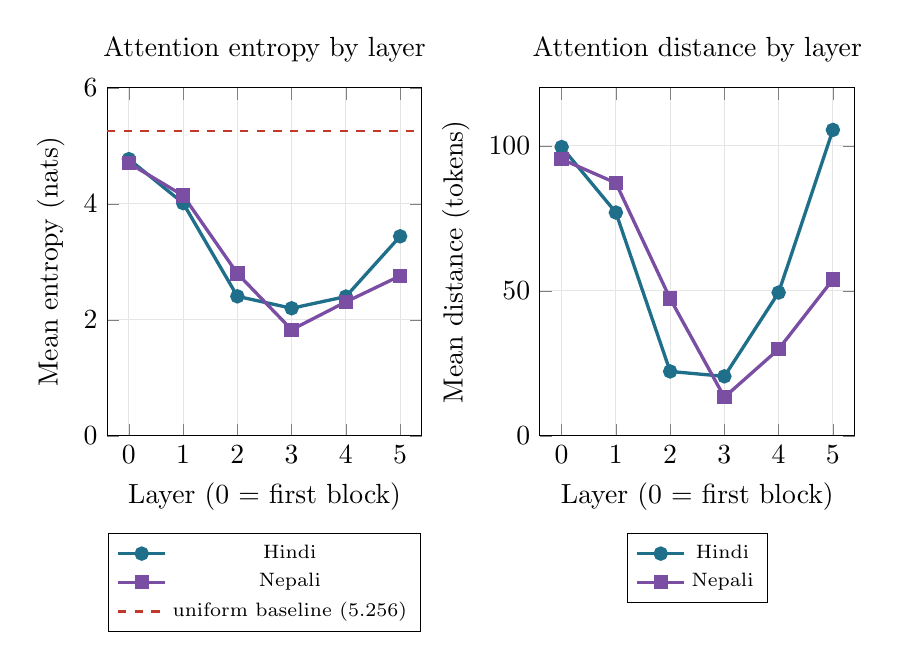
\begin{tikzpicture}
\begin{axis}[
  name=ent,
  width=0.46\textwidth, height=6cm,
  title={Attention entropy by layer},
  xlabel={Layer (0 = first block)}, ylabel={Mean entropy (nats)},
  xmin=-0.4, xmax=5.4, ymin=0, ymax=6,
  xtick={0,1,2,3,4,5},
  grid=both, grid style={gray!20},
  legend style={font=\scriptsize,at={(0.5,-0.28)},anchor=north,legend columns=1},
]
\addplot[hindiblue,very thick,mark=*] coordinates{(0,4.771)(1,4.012)(2,2.405)(3,2.199)(4,2.401)(5,3.440)};
\addlegendentry{Hindi}
\addplot[nepalipurple,very thick,mark=square*] coordinates{(0,4.702)(1,4.143)(2,2.798)(3,1.829)(4,2.309)(5,2.758)};
\addlegendentry{Nepali}
\addplot[warnred,dashed,thick] coordinates{(-0.4,5.2565)(5.4,5.2565)};
\addlegendentry{uniform baseline (5.256)}
\end{axis}
\begin{axis}[
  at={(ent.east)}, anchor=west, xshift=15mm,
  width=0.46\textwidth, height=6cm,
  title={Attention distance by layer},
  xlabel={Layer (0 = first block)}, ylabel={Mean distance (tokens)},
  xmin=-0.4, xmax=5.4, ymin=0, ymax=120,
  xtick={0,1,2,3,4,5},
  grid=both, grid style={gray!20},
  legend style={font=\scriptsize,at={(0.5,-0.28)},anchor=north,legend columns=1},
]
\addplot[hindiblue,very thick,mark=*] coordinates{(0,99.6)(1,77.0)(2,22.2)(3,20.5)(4,49.4)(5,105.5)};
\addlegendentry{Hindi}
\addplot[nepalipurple,very thick,mark=square*] coordinates{(0,95.4)(1,87.2)(2,47.3)(3,13.3)(4,29.9)(5,53.9)};
\addlegendentry{Nepali}
\end{axis}
\end{tikzpicture}
\caption{Both models follow the same shape: layer 0 is diffuse and long-range,
the middle layers sharpen and localise, and layer 5 opens out again. Entropy well
below the red baseline means the heads are selecting, not averaging.}
\label{fig:attnstats}
\end{figure}

\section{The finding worth leading with}

\begin{center}
\begin{tabular}{ccc}
\toprule
Layer & Sharpest head, Hindi & Sharpest head, Nepali \\
& (entropy @ distance) & (entropy @ distance) \\
\midrule
0 & 4.16 @ 45.8 & 3.90 @ 36.0 \\
1 & 3.09 @ 21.9 & 3.17 @ 17.1 \\
2 & 1.49 @ \phantom{0}7.6 & 1.81 @ 10.6 \\
3 & \textbf{0.06 @ \phantom{0}1.3} & \textbf{0.14 @ \phantom{0}1.1} \\
4 & 1.49 @ 22.4 & 1.32 @ \phantom{0}5.6 \\
5 & 2.99 @ 151.4 & 2.48 @ 81.3 \\
\bottomrule
\end{tabular}
\end{center}

\begin{concept}{Both models independently found a "previous-token head"}
Look at layer 3. In \emph{both} models there is a head with entropy almost zero
and distance almost exactly 1.

Entropy 0.06 means the distribution is essentially one-hot --- all the weight on
a single token. Distance 1.3 means that token is the one immediately before.

This head does one job: \textbf{look at the previous word}. It is a well-known
structure in Transformers, and I did not design it or ask for it --- it emerged
from training.

\textbf{Why this is a strong result:} the two models were trained on different
languages, with different tokenizers, different vocabularies, different data and
different random seeds. They shared no weights and no code at runtime. Yet both
arrived at the same organisation. That is good evidence the structure is driven
by the language-modelling objective itself, not by anything specific to one
corpus.
\end{concept}

\begin{concept}{The three-stage story}
\textbf{Layer 0 --- broad.} Entropy 4.7--4.8, distance $\approx$ 100. At this
point each token's vector is basically just "which word am I", with no context, so
there is nothing useful to be selective about. Heads pool broadly.

\textbf{Layers 2--4 --- sharp and local.} Entropy drops to 1.8--2.8, distance to
13--47. Now the vectors carry some context, and heads start doing specific jobs:
tracking the previous token, tracking agreement within a phrase.

\textbf{Layer 5 --- long-range again.} Distance rises to 105 (Hindi), with
individual heads reaching 151 tokens. But entropy stays moderate rather than
minimal, which is the signature of \emph{content-based} attention: choosing among
many distant positions based on what they contain, rather than pointing at a fixed
offset. This is the layer assembling the context needed for the actual prediction.
\end{concept}

\section{How the two models differ}

Hindi attends about 15\% further on average (62.4 vs 54.5 tokens).

\begin{notebox}[But be careful with that comparison]
Before claiming Model H "looks further", remember the tokenizer difference. Model
L's tokens carry 11.44 bytes each versus Model H's 8.88. So 54.5 Nepali tokens
covers roughly the same amount of \emph{text} as 62.4 Hindi tokens.

Converted to bytes, the two mean distances are within about 10\% of each other.
So most of the apparent difference is, once again, a tokenizer effect rather than
a difference in what the models learned.

Noticing this is the kind of care that distinguishes a good analysis from a
superficial one --- the same trap as perplexity, in a different costume.
\end{notebox}

\section{The heatmaps}

Four heatmaps are committed: layer 0 and layer 5, four heads each, for both
models. They plot query position (vertical) against key position (horizontal),
with colour showing attention probability.

Everything above the diagonal is black --- that is the causal mask, visible.

\textbf{Layer 0} shows broad horizontal bands: many queries attending to similar
wide regions. \textbf{Layer 5} shows structure --- bright columns where many query
positions all concentrate on a few informative keys.

The example sentences behind them are stored as text in the attention JSONs, so
the figure remains interpretable even if the font used to render it lacked
Devanagari:

\begin{quote}
\textbf{Hindi:} \dn{किए थे । २०० वर्षों तक जमे हुए ब्रिटिश शासन को 'भारत छोड़ो' के उद्घोष से भगा देना विश्व के इतिहास का गौरवपूर्ण परिवर्तन है ।}

\textbf{Nepali:} \dn{अनुसार नयाँ वर्ष मनाउन चीन गएका उनीहरु त्यसपछि फर्किएका छैनन् । चीन गएकामध्ये एकजना परियोजना...}
\end{quote}

% =======================================================================
\chapter{Everything That Broke, and What It Taught Me}
% =======================================================================

This chapter exists because vivas reward honesty and understanding far more than
a claim that everything worked first time. Each of these is a real failure with a
real diagnosis.

\begin{center}
\begin{longtable}{p{0.30\textwidth}p{0.62\textwidth}}
\toprule
\textbf{What broke} & \textbf{What was actually wrong, and the lesson} \\
\midrule
\endhead
Notebook died instantly on Kaggle &
My notebook generator stripped the newlines from each cell's source, so Jupyter
joined every line into one: \p{import os, sys, json, shutil, subprocess,
timefrom pathlib import Path...}. Worse, my \emph{validator} re-added newlines
before checking, so it was validating a string the notebook never contained.
\textbf{Lesson: validate the artifact exactly as the consumer will read it.} \\
\addlinespace
GPU allocated but unusable &
Kaggle gave me a Tesla P100. \p{torch.cuda.is\_available()} returned True, and
then every kernel launch failed: the P100 is Pascal (sm\_60) and current PyTorch
has dropped Pascal support. \textbf{Lesson: "available" is not "usable".} I
switched to the T4 (sm\_75) and added a check that rejects any compute capability
below 7.0 by name, then runs a real matmul to prove the device works. \\
\addlinespace
Could not find its own data &
I searched \p{/kaggle/input/lma-code} directly. Kaggle actually nests mounts as
\p{/kaggle/input/datasets/<owner>/<slug>/}. \textbf{Lesson: find things by
content, not by path.} Discovery now walks the tree looking for the directory
that contains both language packages. \\
\addlinespace
Evaluation produced nothing &
\p{ModuleNotFoundError: No module named 'sacrebleu'}. Kaggle's image does not
ship it and my notebook never installed requirements. Training was fine --- only
the metrics were lost. \textbf{Lesson: an 11-hour job should verify its
dependencies in the first 10 seconds, not the last 10 minutes.} \\
\addlinespace
Evaluated with the wrong code &
My evaluation kernel loaded \p{hindi/} and \p{nepali/} from the \emph{training
run's own saved output}, not from the code dataset --- so it silently ran an older
revision. \textbf{Lesson: the most dangerous bug is the one that produces
plausible numbers.} Discovery now ranks the code dataset first. \\
\addlinespace
Learning rate silently pinned &
On resume, the schedule restored its \emph{horizon} from the checkpoint, so
extending a run left it computing "progress $>$ 100\%" and clamping to the floor.
Training would have looked stalled with no error. \textbf{Lesson: restore
progress, not policy.} \\
\addlinespace
A rejected job reported success &
The Kaggle CLI exits 0 even when the server refuses the push, so "Maximum batch
GPU session count reached" was being read as a successful launch. \textbf{Lesson:
trust the message, not the exit code.} \\
\bottomrule
\end{longtable}
\end{center}

\begin{notebox}[How to use this chapter in a viva]
If asked "what went wrong?", do not say "nothing". Pick the P100 one or the
stale-code one --- both show real diagnostic reasoning, and the stale-code bug in
particular shows awareness that a wrong-but-plausible result is more dangerous
than a crash.
\end{notebox}

% =======================================================================
\chapter{Strict Check Against the Assignment}
\label{ch:compliance}
% =======================================================================

Every requirement in the Phase 2 specification, checked against files that are
actually in the repository.

\section{Architecture requirements}

\begin{center}
\begin{longtable}{p{0.46\textwidth}p{0.40\textwidth}c}
\toprule
\textbf{Required} & \textbf{Where} & \textbf{Done} \\
\midrule
\endhead
Token embeddings $(V \times d)$ & \p{GPT.token\_embedding} & yes \\
Positional embeddings; state which and why; explain the length limit &
\p{GPT.position\_embedding}, learned absolute; limit explained & yes \\
Combine by addition + embedding dropout & \p{GPT.forward} & yes \\
Project to $Q$, $K$, $V$ & \p{W\_q}, \p{W\_k}, \p{W\_v} (separate Linears) & yes \\
Explicit reshape to $(B,h,T,d_k)$ and back & commented at each transpose & yes \\
Scaled dot-product; explain $1/\sqrt{d_k}$ & \p{/ math.sqrt(head\_dim)} & yes \\
Causal mask, self-implemented & \p{triu} buffer + \p{masked\_fill(-inf)} & yes \\
\textbf{Empirically verify no future leakage} & test measures \textbf{0.000e+00} & yes \\
Concatenate heads, output projection $W_O$ & \p{W\_o} & yes \\
Feed-forward, two linears, non-linearity, wider inside & $512\to2048\to512$, GELU & yes \\
Residual connections around both sublayers & \p{x = x + ...} twice & yes \\
LayerNorm; state pre- or post-norm and why & pre-norm, justified & yes \\
Dropout on attention probabilities and sublayer outputs & three dropouts & yes \\
$N$ blocks then a final normalisation & 6 blocks + \p{ln\_f} & yes \\
Linear head to vocabulary; state tying and the saving & tied; 4.10M / 5.12M saved & yes \\
Cross-entropy at $t$ against token $t{+}1$ & verified slice offsets & yes \\
No \p{nn.Transformer*} / HuggingFace / pre-built attention & AST-checked; only
\p{Linear}, \p{Embedding}, \p{Dropout}, \p{Module}, \p{ModuleList},
\p{Parameter}, \p{init} & yes \\
\bottomrule
\end{longtable}
\end{center}

\section{Pretraining requirements}

\begin{center}
\begin{tabular}{p{0.46\textwidth}p{0.42\textwidth}c}
\toprule
\textbf{Required} & \textbf{Where} & \textbf{Done} \\
\midrule
AdamW & \p{configure\_optimizers} & yes \\
Learning-rate scheduling & cosine + 500-step warmup & yes \\
Validation during training & every 500 steps & yes \\
Checkpoint with weights, optimizer, scheduler, step, config & all present, plus
RNG state & yes \\
Do not initialise one model from the other & separate output dirs, separate seeds & yes \\
About 500M tokens per model & 475.8M / 473.2M & yes \\
\bottomrule
\end{tabular}
\end{center}

\section{The eight deliverables}

\begin{center}
\begin{longtable}{cp{0.40\textwidth}p{0.36\textwidth}}
\toprule
\# & \textbf{Deliverable} & \textbf{Where it lives} \\
\midrule
\endhead
1 & Transformer implementation & \p{*/model/transformer.py} \\
2 & Model configuration files & \p{*/configs/model.yaml} \\
3 & Parameter counts, training scripts, checkpoint links &
    report §1; \p{*/train/train.py}; Drive links in README \\
4 & Training logs and loss curves &
    \p{report/phase2/*\_training\_log.jsonl}, \p{figures/loss\_curves\_both*.png} \\
5 & PPL / BPB tables; BLEU, chrF, ROUGE-L &
    report §4--5, \p{report/phase2/*\_eval.json} \\
6 & Generated samples; diversity / repetition &
    report §5.2; \p{*\_eval.json} $\to$ \p{generation.samples} \\
7 & Attention heatmaps; entropy / distance &
    \p{figures/*\_attention\_layer\{0,5\}.png}, \p{*\_attention.json} \\
8 & Resource-level comparison write-up & report §7 \\
\bottomrule
\end{longtable}
\end{center}

\section{What I did not do, and why}

\begin{warnbox}[Be ready to volunteer these]
\begin{enumerate}[leftmargin=*]
\item \textbf{The bonus ablation (no positional embeddings) was not run.} It
      needs a full 11-hour training run and the two main runs consumed the entire
      30-hour weekly GPU quota. The code supports it --- \p{pos\_encoding: none}
      is a one-line config change, and a test already covers that path --- but the
      run itself did not happen.
\item \textbf{Neither run finished all 15,000 steps.} 14,520 and 14,440, because
      the 11-hour session budget fired first. Reported as-run.
\item \textbf{Intrinsic metrics cover 2M-token subsets} of each split, not the
      full 10.1M / 57.7M test sets. Both models use the identical budget, so the
      comparison is fair, but the numbers are not over the entire split.
\item \textbf{Final evaluation ran on CPU} for both models. Temperature sampling
      draws on device RNG, so evaluating one model on GPU and the other on CPU
      would not have been strictly comparable. Re-running both on the same device
      was the fix.
\item \textbf{Model L's tokenizer has no byte fallback}, giving a 0.17\%
      unknown-token rate. This is inherited from Phase 1 and was deliberately not
      corrected, because the tokenizer is itself a graded Phase 1 artifact.
      Model H's rate is exactly zero.
\end{enumerate}
\end{warnbox}


% =======================================================================
\chapter{Expected Viva Questions, With Answers}
\label{ch:viva}
% =======================================================================

These are the questions I think are most likely, grouped by area. The answers are
written the way I would actually say them out loud.

\section{Architecture --- the most likely area}

\begin{qabox}{Walk me through your forward pass.}
Token ids come in, shape $(32, 512)$. They index the embedding table and become
$(32, 512, 512)$ --- batch, time, model dimension. I add the positional embedding
so the model knows the order, then apply dropout.

That goes through six identical blocks. Each block does two things: masked
multi-head self-attention, then a feed-forward network, each wrapped in a residual
connection with a LayerNorm on the branch.

After the six blocks there is a final LayerNorm, then a linear layer that maps 512
down to the vocabulary size, giving a score for every possible next token. Loss is
cross-entropy between the prediction at position $t$ and the actual token at
position $t{+}1$.
\end{qabox}

\begin{qabox}{Why do you divide by the square root of $d_k$?}
Because without it the softmax saturates.

$Q$ and $K$ start out with roughly unit-size entries. Their dot product sums
$d_k = 64$ such products, so it grows like $\sqrt{d_k}$ --- typical size about 8.
Feeding numbers that large into a softmax makes it nearly one-hot, and a nearly
one-hot softmax has almost no gradient, so learning stalls.

Dividing by $\sqrt{d_k}$ cancels exactly that growth and keeps the scores around
size 1, where softmax is smooth.
\end{qabox}

\begin{qabox}{Show me that your model cannot see the future.}
I have a test for exactly that. It runs the model, saves the logits, then for each
position $t$ changes every token after $t$ and runs again.

The maximum change in the logits at positions $\le t$ is \textbf{0.000e+00} ---
exactly zero, not just small. That is because $\text{softmax}(-\infty)$ is exactly
zero and zero times anything is exactly zero, so masked positions contribute
nothing at all.

The test also checks that the logits \emph{after} $t$ did change --- otherwise a
model that ignored its input entirely would also pass.
\end{qabox}

\begin{qabox}{What would break if you removed the causal mask?}
The model would see the answer. When predicting position 5 it could just look at
position 6 and copy it. Training loss would collapse to near zero and validation
loss would look wonderful --- but at generation time there is no future to read,
so the model would produce nonsense.

It is a particularly nasty bug because all the numbers look better, not worse.
\end{qabox}

\begin{qabox}{Why pre-norm rather than post-norm?}
In post-norm the LayerNorm sits on the residual path itself. In pre-norm it sits
on the branch, so the residual path from the embeddings to the output head is a
clean chain of additions.

That clean path means gradients reach the early layers without being repeatedly
rescaled, which makes training much more forgiving. Deep post-norm stacks are
famous for needing careful warmup or they diverge.
\end{qabox}

\begin{qabox}{Why do you need contiguous() before view()?}
\p{transpose} does not move data --- it only changes the strides, the bookkeeping
that says how far to step in memory. \p{view} needs the data laid out in one
unbroken run. After a transpose it is not, so \p{contiguous()} physically copies
it into the right order first.
\end{qabox}

\begin{qabox}{What is weight tying and what does it save?}
The input embedding is $(V, d)$ and the output head is $(d, V)$ --- same shape,
transposed. Tying means using one matrix for both.

It saves $V \times d$ parameters: 4,096,000 for Hindi, about 18\% of the model,
and 5,120,000 for Nepali, about 21\%. It also forces a token's input and output
representations to be the same vector, which is a sensible constraint.
\end{qabox}

\begin{qabox}{Why 8 heads? Why not 1, or 64?}
One head can really only learn one kind of relationship. Language has many at
once --- subject-verb agreement, what a pronoun refers to, simple adjacency. Eight
heads let eight different patterns be learned in parallel.

Too many heads and each gets too narrow: with $d = 512$, 64 heads would give each
just 8 dimensions to work with, which is not enough to represent much.

My attention analysis shows the specialisation really happened --- layer 3 has a
head that does nothing but look at the previous token, while layer 5 has heads
reaching 151 tokens back.
\end{qabox}

\begin{qabox}{Where does the number 23 million come from?}
Each block is about 3.15M: $4 \times 512^2$ for the four attention projections,
plus $2 \times 512 \times 2048$ for the feed-forward. Six blocks is 18.9M. Add the
token embedding, $8000 \times 512 = 4.1$M, and the positional table,
$512 \times 512 = 0.26$M. Total 23.27M.

The output head costs nothing because it is tied.
\end{qabox}

\section{Training}

\begin{qabox}{Why warmup?}
Adam estimates the mean and variance of each parameter's gradient from a running
average. For the first few hundred steps those estimates are unreliable, and
taking full-size steps based on unreliable estimates is a classic way to diverge
immediately. Warmup ramps the learning rate up over 500 steps while the estimates
settle.
\end{qabox}

\begin{qabox}{What is gradient accumulation, and why did you need it?}
I wanted an effective batch of 32,768 tokens, but that does not fit in memory in
one pass. So I do two forward/backward passes of half that size, add the
gradients, and take one optimizer step. Mathematically identical to one big batch;
half the peak memory.

It is the knob that separates "the batch the maths sees" from "what the GPU can
hold".
\end{qabox}

\begin{qabox}{Your checkpoint --- what is in it, and why each piece?}
Weights, optimizer state, scheduler state, step number, tokens consumed, best
validation loss, the full config, and both RNG states.

The optimizer state matters most after the weights: Adam's momentum estimates take
hundreds of steps to rebuild, so dropping them causes a visible loss spike on
resume. Scheduler state keeps the learning rate continuing rather than restarting
warmup. RNG state keeps the data order identical.

I verified resume across three consecutive sessions before the real runs.
\end{qabox}

\begin{qabox}{Did anything go wrong with resume?}
Yes, and the test caught it. When I resumed with a larger step budget, the
schedule restored its \emph{horizon} from the checkpoint as well as its position.
So it thought it was already past the end, computed progress above 100\%, and
pinned the learning rate at the floor for the whole extension. Training would have
looked stalled with no error at all.

The fix was to restore only the progress and take the schedule's shape from the
live config, printing a warning when they differ.
\end{qabox}

\begin{qabox}{Why is your validation loss lower than your training loss?}
Because dropout is on during training and off during evaluation. The training
number is measured on a deliberately handicapped model, so it is expected to look
slightly worse. It is not a sign of anything wrong.
\end{qabox}

\section{Evaluation --- prepare hardest for this}

\begin{qabox}{Which model is better?}
It depends on the metric, and that is the interesting part.

By perplexity, Model H is better by 41 percent --- 27.4 against 46.7. By
bits-per-byte, Model L is actually slightly ahead --- 0.485 against 0.538.

They disagree because perplexity is measured per token, and the two tokenizers
produce very different tokens. Nepali's tokens carry 11.44 bytes of text each
against Hindi's 8.88, so Model L is being asked a harder question at every step.

Bits-per-byte divides by bytes of actual text instead, which removes the tokenizer
from the comparison. On that measure the two models are close.

So my answer is: most of the apparent gap is a tokenizer artifact, not a real
quality difference. If I had reported perplexity alone I would have drawn the
wrong conclusion.
\end{qabox}

\begin{qabox}{So the lower-resource model is better?}
No, I would not claim that. The bits-per-byte difference is small, and both models
have limitations. What I would claim is narrower and more defensible: the
\emph{41 percent gap that perplexity suggests is not real}. On the
tokenizer-neutral measure they are close.
\end{qabox}

\begin{qabox}{Your bits-per-byte of 0.48 is better than published English models. Explain.}
That comparison is not valid, and I would not make it. Devanagari costs three
UTF-8 bytes per character, whereas most English characters cost one. So the byte
denominator is roughly three times larger for the same amount of text, which
mechanically lowers the number.

My BPB figures are comparable Hindi against Nepali, because both are Devanagari.
They cannot be compared against a Latin-script model.
\end{qabox}

\begin{qabox}{Your BLEU is under 2. Is your model broken?}
No. BLEU counts exact four-word matches against a single reference continuation.
For open-ended text there are many valid continuations and the model's is unlikely
to match the one true one word-for-word, so BLEU sits near the floor regardless of
quality.

It is only useful relatively --- comparing decoding settings of the same model.
The metric I actually trust here is chrF++, which compares character n-grams and
therefore handles the rich inflection in both languages. It peaks at temperature
1.0, which is also where the text reads best.
\end{qabox}

\begin{qabox}{Why did you implement ROUGE-L yourself?}
Because the standard \p{rouge\_score} library's default tokenizer lowercases the
text and strips characters that are not ASCII alphanumeric. On Devanagari that
deletes the entire string and silently returns zero.

So I compute the longest common subsequence over whitespace tokens directly. It is
a small amount of code and it actually works on the script I am using.
\end{qabox}

\begin{qabox}{Your greedy decoding repeats itself. Why?}
Once the model emits a word, that word is in its own context, which makes the same
word slightly more likely next time. Greedy always takes the maximum, so the loop
tightens and never breaks. My greedy repetition rate is 59.8 percent of 4-grams.

Sampling fixes it because there is always a chance of choosing something else. At
temperature 1.0 the repetition rate drops to 0.2 percent, and chrF++ improves at
the same time --- so up to that point the diversity costs nothing in quality.
\end{qabox}

\section{Attention analysis}

\begin{qabox}{What did your attention heads learn?}
Three stages, and both models found the same one independently.

Layer 0 is diffuse and long-range --- entropy near 4.8, distance around 100. At
that point the token vectors have no context yet, so there is nothing useful to be
selective about.

Layers 2 to 4 sharpen and localise. Layer 3 in both models contains a head with
entropy 0.06 and distance 1.3 --- essentially one-hot, pointing at the immediately
previous token. That is a previous-token head, and it emerged on its own.

Layer 5 opens out again, with distance over 100 and individual heads reaching 151
tokens, but with moderate rather than minimal entropy. That pattern --- far but not
sharp --- is the signature of content-based attention: choosing among many distant
positions by what they contain.
\end{qabox}

\begin{qabox}{How do you know the entropy number means anything?}
Because I compare it against a baseline. A head that spread its attention
perfectly evenly over a 512-token causal window would have entropy 5.256 nats. My
models measure 3.205 and 3.090, about 2 nats below that.

I also checked an untrained model: it measured 3.2558 against a baseline of
3.2566 on a shorter sequence --- indistinguishable from uniform, exactly as it
should be. So the gap in the trained models is a real learned effect.
\end{qabox}

\begin{qabox}{Model H attends further than Model L. What does that tell you?}
Less than it first appears. Hindi averages 62.4 tokens and Nepali 54.5, so about
15 percent further.

But Nepali's tokens carry more text --- 11.44 bytes against 8.88. Converting to
bytes, the two distances come within about 10 percent of each other. So most of
that difference is the same tokenizer effect that distorted perplexity, wearing a
different costume. I would not claim the models learned meaningfully different
context ranges.
\end{qabox}

\section{Design and process}

\begin{qabox}{Why are your two models the same size? Was that not a constraint?}
It was a deliberate choice, and it is the reason the comparison means anything.

The non-embedding parameter counts are exactly equal --- 18,915,328 --- and the
token budgets differ by 0.55 percent. So if Model H does better, it cannot be
because it was bigger or trained longer. The only things that differ are the data
and the tokenizer, which is exactly what the phase is meant to study.
\end{qabox}

\begin{qabox}{Your two language directories contain identical code. Is that not duplication?}
It is, and it was deliberate. The specification says to organise the repository by
language with each language directory self-contained. I originally had a shared
package, which satisfied the independence rule but left \p{hindi/model/} and
\p{hindi/train/} empty --- the exact directories the specification's example layout
says should hold the code.

So each language now has its own copy. They are independent packages: neither
imports the other, and each can be run, read or graded on its own. The cost is
that a bug fix has to be applied twice, which I accepted for the clarity.
\end{qabox}

\begin{qabox}{What was the hardest part?}
Honestly, the infrastructure rather than the model. The Transformer itself is well
specified --- if the shapes line up and the mask test passes, it is right.

The hard part was a category of bug where things look like they are working. The
worst was my evaluation kernel loading the code from the training run's own saved
output instead of the code dataset, so it silently ran an older revision and
produced plausible but wrong numbers. A crash is easy. A wrong answer that looks
right is what you have to design against.
\end{qabox}

\begin{qabox}{If you had more compute, what would you do?}
Three things, in order.

First, finish the 15,000 steps --- both runs stopped around 14,500 when the time
budget fired, and both loss curves were still descending.

Second, run the positional-embedding ablation. The code already supports it as a
one-line config change; I ran out of GPU quota, not capability.

Third, train longer overall. At 23 million parameters and 476 million tokens
neither model is close to overfitting, so more data passes would still help.
\end{qabox}

\begin{qabox}{What would you do differently?}
Check dependencies at the start of a long job rather than at the end. I lost an
evaluation because \p{sacrebleu} was missing on Kaggle, and that was discovered
after eleven hours of training rather than in the first ten seconds. Training was
fine and I could re-run the evaluation cheaply, but it was avoidable.
\end{qabox}

% =======================================================================
\chapter{One-Page Cheat Sheet}
\label{ch:cheatsheet}
% =======================================================================

\section{Numbers to know cold}

\begin{center}
\begin{tabular}{lrr}
\toprule
& \textbf{Model H (Hindi)} & \textbf{Model L (Nepali)} \\
\midrule
Vocabulary & 8,000 Unigram & 10,000 BPE \\
Total parameters & 23,273,472 & 24,297,472 \\
Non-embedding parameters & \multicolumn{2}{c}{\textbf{18,915,328 --- identical}} \\
Layers / heads / $d$ / $d_{ff}$ & \multicolumn{2}{c}{6 / 8 / 512 / 2048} \\
Context length & \multicolumn{2}{c}{512} \\
Steps completed & 14,520 & 14,440 \\
Training tokens & 475,791,360 & 473,169,920 \\
Throughput & \multicolumn{2}{c}{12.0k tokens/sec on a Tesla T4, 11 hours each} \\
\midrule
Validation perplexity & \textbf{27.07} & 46.14 \\
Test perplexity & \textbf{27.41} & 46.68 \\
Test bits-per-byte & 0.5382 & \textbf{0.4846} \\
Bytes per token & 8.88 & 11.44 \\
\midrule
Mean attention entropy & 3.205 & 3.090 \\
Uniform baseline & \multicolumn{2}{c}{5.256} \\
Mean attention distance & 62.4 & 54.5 \\
Previous-token head (layer 3) & 0.06 @ 1.3 & 0.14 @ 1.1 \\
\midrule
Causal-mask leakage & \multicolumn{2}{c}{\textbf{0.000e+00}} \\
Initial loss vs $\ln V$ & \multicolumn{2}{c}{8.98 vs 8.987} \\
\bottomrule
\end{tabular}
\end{center}

\section{The four things to say if given an open question}

\begin{enumerate}[leftmargin=*]
\item \textbf{Perplexity and bits-per-byte disagree, and that is the finding.}
      Perplexity favours Hindi by 41\%; BPB puts Nepali slightly ahead. The gap is
      mostly a tokenizer artifact --- Nepali's tokens carry 11.44 bytes against
      8.88. Reporting perplexity alone would have given the wrong conclusion.
\item \textbf{The comparison is controlled.} Non-embedding parameters exactly
      equal, token budgets within 0.55\%. So differences come from data and
      tokenizer, not size or compute.
\item \textbf{Both models independently learned the same attention structure},
      including a previous-token head at layer 3 --- different languages,
      tokenizers and seeds.
\item \textbf{The causal mask is provably correct}: leakage measured at exactly
      0.000e+00, with a converse check so a model ignoring its input could not
      pass.
\end{enumerate}

\section{Formulas}

\begin{align*}
\text{Attention}(Q,K,V) &= \text{softmax}\!\left(\frac{QK^\top}{\sqrt{d_k}} + M\right)V \\[4pt]
\text{Perplexity} &= e^{\text{cross-entropy in nats}} \\[4pt]
\text{Bits-per-byte} &= \frac{\text{cross-entropy in nats} / \ln 2}{\text{bytes per token}} \\[4pt]
\text{Parameters per block} &\approx 12 d^2 \quad (4d^2 \text{ attention} + 8d^2 \text{ FFN})
\end{align*}

\section{Where everything lives}

\begin{center}
\begin{tabular}{ll}
\toprule
What & Path \\
\midrule
Transformer & \p{hindi/model/transformer.py}, \p{nepali/model/transformer.py} \\
Config & \p{*/configs/model.yaml} \\
Training loop & \p{*/train/train.py} \\
Evaluation & \p{*/eval/evaluate.py} \\
Attention analysis & \p{*/eval/attention.py} \\
Plots & \p{*/eval/viz.py} \\
Causal-mask proof & \p{*/tests/test\_model.py} \\
Graded report & \p{report/phase2/phase2\_report.md} \\
All results & \p{report/phase2/} \\
Checkpoints & Google Drive, linked in the README \\
\bottomrule
\end{tabular}
\end{center}

\begin{notebox}[Final advice to myself]
If I do not know something, say so plainly and then say what I would do to find
out. Every examiner prefers that to a confident guess.

And if the conversation stalls, steer it to the perplexity-versus-bits-per-byte
result. It is the most interesting thing in the project, it shows I understood
\emph{why} the assignment asked for both metrics, and I can defend every number in
it.
\end{notebox}

\end{document}
